\documentclass[12pt]{article}

\usepackage{amssymb,amsmath,amsfonts,eurosym,geometry,ulem,graphicx,caption,color,setspace,sectsty,comment,footmisc,caption,natbib,pdflscape,subfigure,array,hyperref}
\usepackage{booktabs}
\usepackage{multirow}
\usepackage{graphicx}
\usepackage{graphicx}
\usepackage{amsmath}
\usepackage{amsfonts}
\usepackage{amssymb}
\usepackage{tikz}
\usetikzlibrary{snakes}
\usepackage{float}
\usepackage{subfigmat}
\usepackage{etoolbox}
\usepackage{amssymb}
\usepackage{caption}
\usepackage{lscape}
\usepackage{graphicx}
\usepackage{pdflscape}
\usepackage{adjustbox}
\usepackage{xcolor}
\usepackage{graphicx}
\usepackage{hyperref}
\usepackage{hyperref}
\normalem

\onehalfspacing
\newtheorem{theorem}{Theorem}
\newtheorem{proposition}{Proposition}
\newenvironment{proof}[1][Proof]{\noindent\textbf{#1.} }{\ \rule{0.5em}{0.5em}}

\newtheorem{hyp}{Hypothesis}
\newtheorem{subhyp}{Hypothesis}[hyp]
\renewcommand{\thesubhyp}{\thehyp\alph{subhyp}}

\newcommand{\red}[1]{{\color{red} #1}}
\newcommand{\blue}[1]{{\color{blue} #1}}

\newcolumntype{L}[1]{>{\raggedright\let\newline\\arraybackslash\hspace{0pt}}m{#1}}
\newcolumntype{C}[1]{>{\centering\let\newline\\arraybackslash\hspace{0pt}}m{#1}}
\newcolumntype{R}[1]{>{\raggedleft\let\newline\\arraybackslash\hspace{0pt}}m{#1}}

\geometry{left=1.0in,right=1.0in,top=1.0in,bottom=1.0in}

\begin{document}

\begin{titlepage}
\title{GSF-3100 \\ Marchés des Capitaux}
\date{\today}
\maketitle

\setcounter{page}{0}
\thispagestyle{empty}
\end{titlepage}
\pagebreak \newpage

\tableofcontents
\pagebreak \newpage

\chapter{Mathématiques des Obligations}

\section{Équivalence de taux}
Afin de pouvoir comprendre le fonctionnement d'une obligation, il est important de bien maitriser le concept de taux d'intérêt nominal et effectif.

\begin{itemize}
\item Taux d'Intérêt Effectif (Notation : $r$)
\begin{enumerate}
\item Il s'agit du taux utilisé dans le calcul de la capitalisation et de l'actualisation. 
\item Il s'agit également du taux réellement reçu sur un investissement $P_0$ et rapportant $I$ en intérêt.
\begin{align*}
I=P_0 \times r
\end{align*}
\end{enumerate}
\item Taux d'Intérêt Nominal (Notation : $(i;m)$)
\begin{enumerate}
\item Sera toujours accompagné d'un valeur $m$ représentant le nombre de capitalisation par période.
\item Il ne doit pas être utilisé dans les calculs d’actualisation et de capitalisation
\end{enumerate}
\end{itemize}

Le taux d'intérêt effectif $r$ est une fonction de notre taux d'intérêt nominal $i$ et de notre nombre de capitalisation par période. 
\begin{align*}
r=\frac{i}{m}
\end{align*}
Nous allons maintenant regarder comment effectuer une équivalence de taux. 


\subsection{Taux effectif $\rightarrow$ Taux effectif}

Transformer un taux effectif $r_2$ en un autre taux effectif $r_1$ à l'aide de l'équation suivante:
\begin{align*}
r_1 =(1+r_2)^{\frac{u}{v}}-1
\end{align*}
Sachant 
\begin{itemize}
\item $r_1$ est le taux effectif par $u$ période 
\item $r_2$ est le taux effectif par $v$ période 
\end{itemize}
Voici les valeurs prises par $u$ et $v$ lorsque nous avons les taux effectifs suivants 


\begin{table}[H]
\begin{center}
\begin{tabular}{|c|c|l|l|}
\hline
\multicolumn{1}{|l|}{\textbf{$r_1$}} & \multicolumn{1}{l|}{\textbf{$r_2$}} & \textbf{$u$} & \textbf{$v$} \\ \hline
\textbf{Quotidien}                   & \textbf{Annuel}                     & 1            & 365          \\ \hline
\textbf{Hebdomadaire}                & \textbf{Annuel}                     & 1            & 52           \\ \hline
\textbf{Mensuel}                     & \textbf{Annuel}                     & 1            & 12           \\ \hline
\textbf{Trimestriel}                 & \textbf{Annuel}                     & 1            & 4            \\ \hline
\textbf{Semestriel}                  & \textbf{Annuel}                     & 1            & 2            \\ \hline
\textbf{Quotidien}                   & \textbf{Semestriel}                 & 2            & 365          \\ \hline
\textbf{Hebdomadaire}                & \textbf{Semestriel}                 & 2            & 52           \\ \hline
\textbf{Mensuel}                     & \textbf{Semestriel}                 & 2            & 12           \\ \hline
\textbf{Trimestriel}                 & \textbf{Semestriel}                 & 2            & 4            \\ \hline
\end{tabular}
\end{center}
\end{table}

\subsection{Taux effectif $\rightarrow$ Taux nominal}
Transformer un taux effectif $r$ en un taux nominal $(i;m)$ à l'aide de l'équation suivante:
\begin{align*}
i = r \times m
\end{align*}

\subsection{Taux nominal $\rightarrow$ Taux effectif}
Transformer un taux nominal $(i;m)$ en un taux effectif $r$ à l'aide de l'équation suivante:
\begin{align*}
r=\frac{i}{m}
\end{align*}

\pagebreak \newpage

\section{Capitalisation et Actualisation}
\subsection{Valeur Future (Capitalisation)}
Dans cette section, nous allons regarder comment capitaliser un montant unique. La capitalisation nous permet de déterminer la valeur future d'un montant d'argent investit aujourd'hui à un taux spécifié. Voici les paramètres que nous utiliserons:
\begin{itemize}
\item $P_0=$ Montant investi en $t=0$ 
\item $r=$ Taux d'intérêt périodique reçu sur l'investissement
\item $n=$ Période pendant lequel le montant initial est investi
\item $P_n=$ Valeur future de notre investissement $P_0$ en $t=n$
\end{itemize}

Voici l'équation nous permettant de trouver la valeur future de notre investissement 
\begin{align*}
P_n=P_0 \times (1+r)^n
\end{align*}

\subsection{Valeur Présente (Actualisation)}
Dans cette section, nous allons regarder comment actualiser un montant unique. L'actualisation nous permet de déterminer la valeur présente d'un montant d'argent que nous allons recevoir dans le future. Voici les paramètres que nous utiliserons:
\begin{itemize}
\item $P_0=$ Montant à recevoir dans le futur en valeur d'aujourd'hui ($t=0$), soit la valeur présente  
\item $r=$ Taux d'intérêt périodique en vigueur dans l'économie
\item $n=$ Nombre de périodes avant que le montant soit reçu.
\item $P_n=$ Montant nominal à recevoir dans le futur ($t=n$)
\end{itemize}

Voici l'équation nous permettant de trouver la valeur présente d'un montant à recevoir dans le futur.
\begin{align*}
P_0=\frac{P_n}{(1+r)^n}
\end{align*}

\pagebreak \newpage

\section{Annuité}

Une annuité est tout simplement une suite de paiements identiques et reçus à intervalle constant pendant une période spécifiée. Voici une ligne du temps représentant une annuité.

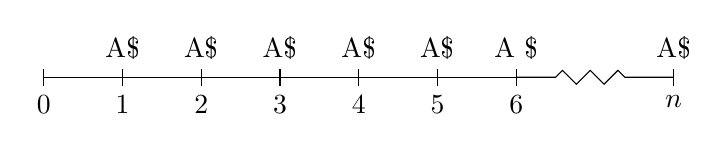
\begin{tikzpicture}[snake=zigzag, line before snake = 5mm, line after snake = 5mm]
    % draw horizontal line   
    \draw (0,0) -- (6,0);
    \draw[snake] (6,0) -- (8,0);

    % draw vertical lines
    \foreach \x in {0,1,2,3,4,5,6,8}
      \draw (\x cm,3pt) -- (\x cm,-3pt);

    % draw nodes
    \draw (0,0) node[below=3pt] {$ 0 $} node[above=3pt] {$   $};
    \draw (1,0) node[below=3pt] {$ 1 $} node[above=3pt] {A\$};
    \draw (2,0) node[below=3pt] {$ 2 $} node[above=3pt] {A\$};
    \draw (3,0) node[below=3pt] {$ 3 $} node[above=3pt] {A\$};
    \draw (4,0) node[below=3pt] {$ 4 $} node[above=3pt] {A\$};
    \draw (5,0) node[below=3pt] {$ 5 $} node[above=3pt] {A\$};
    \draw (6,0) node[below=3pt] {$ 6 $} node[above=3pt] {A \$};
    \draw (7,0) node[below=3pt] {$  $} node[above=3pt] {$  $};
    \draw (8,0) node[below=3pt] {$ n $} node[above=3pt] {A\$};
  \end{tikzpicture}

\begin{itemize}
\item $A\$$ représente le paiement reçu à chaque période 
\item $n$ représente le nombre de paiements que versera l'annuité
\end{itemize}

\subsection{Valeur future d'une annuité régulière}

La valeur future d'une annuité régulière, nous donnera la valeur de la somme de tous les flux $A\$$ capitalisé à $t=n$. $VF_{P_n}$ sera la notation que nous utiliserons pour la valeur future d'une annuité régulière. L'équation suivante montre comment obtenir la valeur future de notre annuité régulière.  
\begin{align*}
VF_{P_n} = A \times (1+r)^{n-1}+A \times (1+r)^{n-2}+....+A \times (1+r)^{1}+A \times (1+r)^{0}
\end{align*}
Si le nombre de période $n$ est relativement faible, il sera simple de calculer la valeur future. Cependant, si nous avons un nombre important de périodes $n$, la formule suivante est plus pratique. 
\begin{align*}
VF_{P_n}=A \left[\frac{(1+r)^n-1}{r} \right]
\end{align*}
Sachant les paramètres suivants: 
\begin{itemize}
\item $VF_{P_n}=$ Valeur future d'une annuité régulière 
\item $A=$ flux monétaire constant reçu à chaque période  
\item $n=$ Nombre de flux monétaire qui sera versé dans cette annuité régulière
\item $r=$ taux d'intétêt périodique en vigueur 
\end{itemize}


\subsection{Valeur présente d'une annuité régulière}

La valeur présente d'une annuité régulière, nous donnera la valeur de la somme de tous les flux $A\$$ actualisé en $t=0$. $VP_{P_0}$ sera la notation que nous utiliserons pour la valeur présente d'une annuité régulière. L'équation suivante montre comment obtenir la valeur présente de notre annuité régulière.  
\begin{align*}
VP_{P_0} = \frac{A}{(1+r)^{1}}+\frac{A}{(1+r)^{2}}+....+\frac{A}{(1+r)^{n-1}}+\frac{A}{(1+r)^{n}}
\end{align*}
Si le nombre de période $n$ est relativement faible, il sera simple de calculer la valeur présente. Cependant, si nous avons un nombre important de périodes $n$, la formule suivante est plus pratique. 
\begin{align*}
VP_{P_0}=A \left[ \frac{1-\frac{1}{(1+r)^n}}{r} \right]
\end{align*}
Sachant les paramètres suivants: 
\begin{itemize}
\item $VP_{P_0}=$ Valeur présente d'une annuité régulière 
\item $A=$ flux monétaire constant reçu à chaque période  
\item $n=$ Nombre de flux monétaire qui sera versé dans cette annuité régulière
\item $r=$ taux d'intétêt périodique en vigueur 
\end{itemize}

\subsection{Annuité de début de période}
Si nous sommes en présence d'une annuité de début de période, la ligne du temps sera modifiée comme suit: \\

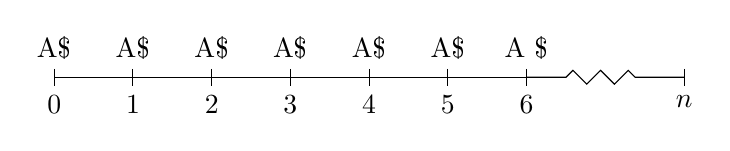
\begin{tikzpicture}[snake=zigzag, line before snake = 5mm, line after snake = 5mm]
    % draw horizontal line   
    \draw (0,0) -- (6,0);
    \draw[snake] (6,0) -- (8,0);

    % draw vertical lines
    \foreach \x in {0,1,2,3,4,5,6,8}
      \draw (\x cm,3pt) -- (\x cm,-3pt);

    % draw nodes
    \draw (0,0) node[below=3pt] {$ 0 $} node[above=3pt] {A\$};
    \draw (1,0) node[below=3pt] {$ 1 $} node[above=3pt] {A\$};
    \draw (2,0) node[below=3pt] {$ 2 $} node[above=3pt] {A\$};
    \draw (3,0) node[below=3pt] {$ 3 $} node[above=3pt] {A\$};
    \draw (4,0) node[below=3pt] {$ 4 $} node[above=3pt] {A\$};
    \draw (5,0) node[below=3pt] {$ 5 $} node[above=3pt] {A\$};
    \draw (6,0) node[below=3pt] {$ 6 $} node[above=3pt] {A \$};
    \draw (7,0) node[below=3pt] {$  $} node[above=3pt] {$ $};
    \draw (8,0) node[below=3pt] {$ n $} node[above=3pt] {$ $};
  \end{tikzpicture}
  
La valeur future et présente d'une annuité de début de période pourra être trouvée en utilisant la formule pour l'annuité régulière avec un ajustement. En effet, la formule pour l'annuité régulière appliquée pour une annuité de début de période capitalisera l'ensemble des flux monétaire à $t=n-1$ pour la valeur future et actualisera l'ensemble des flux monétaire en $t=-1$ pour la valeur présente. Afin de déplacer $VF_{P_n}$ à $t=n$ et $VP_{P_0}$ à $t=0$, il faut multiplier la valeur présente et future de notre annuité régulière par $(1+r)$.

\begin{itemize}
\item Valeur future d'une annuité de début de période $VF_{P_n^*}$
\end{itemize}
\begin{align*}
VF_{P_n^*}=VF_{P_n} \times (1+r)
\end{align*}
\begin{align*}
VF_{P_n^*}=A \left[\frac{(1+r)^n-1}{r} \right] \times (1+r)
\end{align*}

\begin{itemize}
\item Valeur présente d'une annuité de début de période $VP_{P_0^*}$
\end{itemize}
\begin{align*}
VP_{P_0^*}=VP_{P_0} \times (1+r)
\end{align*}
\begin{align*}
VP_{P_0^*}=A \left[ \frac{1-\frac{1}{(1+r)^n}}{r} \right] \times (1+r)
\end{align*}

\newpage
\section{Déterminer le prix d'une obligation}
Dans cette section nous allons regarder comment trouver le prix de trois types d'obligations.
\begin{itemize}
\item Obligation régulière 
\item Obligation Zéro Coupon
\item Obligation perpétuelle
\end{itemize}

\subsection{Obligation régulière}
Dans une obligation régulière un coupon est versé tous les semestres et le calcul du coupon est le suivant:
\begin{align*}
C= M * \frac{TC}{2}
\end{align*}
Où 
\begin{itemize}
\item $C=$ coupon semetriel 
\item $TC=$ taux de coupon annuel 
\item $M=$ Valeur nominal de l'obligation 
\end{itemize}
\vspace{1cm}
Les flux monétaire d'une obligation peuvent être séparés en deux importantes composantes. 

\begin{enumerate}
\item Coupon payé de façon périodique jusqu'à l'échéance
\item Paiement de la valeur à l'échéance
\end{enumerate}
\vspace{1cm}
Le prix d'une obligation peut être également séparé en deux composantes:

\begin{enumerate}
\item la valeur actuelle des paiements de coupons semestriels
\item la valeur actuelle de la valeur à l'échéance 
\end{enumerate}
\vspace{1cm}
Voici l'équation pour trouver le prix d'une obligation régulière:

\begin{align*}
P=\frac{C}{(1+r)^1}+\frac{C}{(1+r)^2}+...+\frac{C}{(1+r)^n}+\frac{M}{(1+r)^n}
\end{align*}

\begin{align*}
P=\sum_{t=1}^{n} \frac{C}{(1+r)^t}+\frac{M}{(1+r)^n}
\end{align*}

On peut donc remarquer la présence d'une annuité dans la dernière équation 
\begin{align*}
\sum_{t=1}^{n} \frac{C}{(1+r)^t}=C \left[ \frac{1-\frac{1}{(1+r)^n}}{r} \right]
\end{align*}
On peut donc arriver à l'équation simplifiée pour le prix d'une obligation régulière.
\begin{align*}
P=C \left[ \frac{1-\frac{1}{(1+r)^n}}{r} \right]+\frac{M}{(1+r)^n}
\end{align*}
\subsection{Obligation Zéro Coupon}
Une obligation zéro coupon à la particularité de ne pas payer de coupons. Une obligation zéro coupon possède comme unique flux monétaire, la valeur actuelle de la valeur à l'échéance. On peut donc trouver le prix d'une obligation zéro coupon en actualisant seulement la valeur à l'écheance $M$. 
\begin{align*}
P_{zc}=\frac{M}{(1+r)^n}
\end{align*}
Où $P_{zc}$ représente le prix d'une obligation zéro coupon au temps $t=0$ venant à échéance après $n$ périodes 
\subsection{Obligation perpétuelle}
Une obligation perpétuelle à la particularité de ne pas avoir d'échéance. En effet, on suppose que les coupons seront payés pendant une période infinie. Sachant cela, il nous possible de dire que la valeur d'une obligation perpétuelle est la suivante.
\begin{align*}
P_{p}=\sum_{t=1}^{\infty} \frac{C}{(1+r)^t}
\end{align*} 
Après manipulation de la dernière équation, il est possible d'arriver à l'expression suivante  pour le prix d'une obligation perpétuelle $P_p$.
\begin{align*}
P_p=\frac{C}{r}
\end{align*}

\section{Intérêt couru et cote}

\subsection{Prix d'une obligation entre deux dates de coupon}
Il faut tout d'abord calculer le prix d'une obligation au moment où le dernier coupon a été versé. Si on suppose que le dernier coupon a été versé en t=0, alors le prix d'une obligation régulière à ce moment est trouvée comme suit:
\begin{align*}
P_0=C \left[ \frac{1-\frac{1}{(1+r)^n}}{r} \right]+\frac{M}{(1+r)^n}
\end{align*}
Le problème est que depuis le dernier coupon, une période de k s'est écoulée, alors le prix que nous venons de calculer est trop faible. Si le détenteur décidait de vendre sont obligation à $t= k$, au prix de $t=0$, il laisserait la totalité du prochain coupon au prochain acheteur. Pour rectifier cette situation, il faut ajuster le prix $P_0$ pour tenir compte de l'intérêt accumulé entre $t=0$ et $t=k$. Il s'agit tout simplement de capitaliser le prix $P_0$ sur $k$ période. 
\begin{align*}
P_k=P_0 (1+r)^k
\end{align*}
Nous obtiendrons ainsi le prix reflétant l'intérêt accumulé $P_k$, appelé \textbf{full price} ou \textbf{dirty price}. On trouve ainsi l'équation complète afin de déterminer le prix d'une obligation entre deux paiements de coupons.
\begin{align*}
P_k= \left( C \left[ \frac{1-\frac{1}{(1+r)^n}}{r} \right]+\frac{M}{(1+r)^n} \right) \times (1+r)^k
\end{align*}
\newpage
\subsection{Cotation}
Nous utiliserons le terme \textbf{cote} où \textbf{clean price} comme étant la valeur de l'obligation servant uniquement à rénumérer le vendeur de l'obligation pour la valeur intrinsèque. Pour trouver  ce prix, il faut soustraire les intérêts courrus au prix $P_k$.
\begin{align*}
cote_k=P_k-IC_k
\end{align*}
Où
\begin{itemize}
\item $cote_k=$ \textbf{clean price} à $t=k$
\item $P_k=$ \textbf{full price} ou \textbf{dirty price} à $t=k$
\item $IC_k=$ Intérêts courus à $t=k$
\end{itemize}

Pour trouver les intérêts courrus, il nous suffit de multiplier $k$ par la valeur du coupon périodique.
\begin{align*}
IC_k= k \times C
\end{align*}
\subsection{Convention pour la valeur de $k$}
Il est important de comprendre que $k$ possède comme unité de mesure, une période de coupon. Pour faciliter la compréhension, si on est exactement à mi-chemin entre deux versements de coupons, la valeur prise par $k$ sera de $0.5$. De façon très générale $k$ est déterminé avec la formule suivante:
\begin{align*}
k= \frac{N_{C_{t}}^{C_{t+k}}}{N_C}
\end{align*}
Où 
\begin{itemize}
\item $N_{C_{t}}^{C_{t+k}}$ est le nombre de jours depuis le dernier coupon. 
\item $N_C$ est le nombre de jours dans une période de coupon. 
\end{itemize}
\newpage
De plus, tout dépendant du type d'obligation, une convention différente pour trouver la valeur de k sera appliquée.
\begin{itemize}
\item Titres gouvernementaux
\begin{align*}
k=\frac{Exact}{Exact}
\end{align*}
\begin{itemize}
\item Numérateur : le nombre de jours exacts depuis le dernier coupon
\item Dénominateur : le nombre de jours exacts dans une période de coupon.
\end{itemize}
\item Marché monétaire américain 
\begin{align*}
k=\frac{Exact}{360}
\end{align*}
\begin{itemize}
\item Numérateur : le nombre de jours exacts depuis le dernier coupon
\item Dénominateur : 360/nombre de coupons par année
\end{itemize}
\item Obligations corporatives 
\begin{align*}
k=\frac{30}{360}
\end{align*}
\begin{itemize}
\item Numérateur : le nombre de jours depuis le dernier coupon en accordant aux mois entiers depuis le dernier coupon une valeur de 30 jours.
\item Dénominateur : 360/nombre de coupons par année
\end{itemize}
\item Autre 
\begin{align*}
k=\frac{Exact}{365}
\end{align*}
\begin{itemize}
\item Numérateur : le nombre de jours exacts depuis le dernier coupon
\item Dénominateur : 365/nombre de coupons par année
\end{itemize}
\end{itemize}

\newpage

\section{Rendement réalisé}
Dans cette section, nous allons définir les étapes afin de calculer le rendement réalisé lorsque nous avons acheté une obligation à $t=0$ ayant une échéance à $t=n$ et que nous l'avons vendue par la suite à $t=m$. De plus nous allons supposer les élèments suivants:
\begin{itemize}
\item Le coupon prendra $C$ comme valeur 
\iten La valeur à l'échéance de l'obligation prendra $M$ comme valeur
\item Les coupons seront réinvestit au taux $r_{réinvestissement}$ 
\item L'obligation sera acheté avec un rendement à l'échéance de $r_{achat}$
\item L'obligation sera vendu à rendement à l'échéance de $r_{vente}$
\item L'obligation versera 2 coupons chaque année, soit de façon semestrielle. 
\end{itemize}

 
Par la suite, nous allons effectuer les 4 étapes suivantes: 
\begin{enumerate}
\item Calculer le prix d'achat en $t=0$
\item Calculer la valeur future des coupons à $t=m$, pour tenir compte du réinvestissement des coupons.
\item Calcul du prix de vente à $t=m$
\item Calcul du rendement réalisé avec les valeurs trouvées dans l'étape 1, 2 et 3.
\end{enumerate}

\subsection{Étape 1}
Voici l'équation qui nous permet de trouver le prix d'achat en $t=0$
\begin{align*}
P_0=C \times \left[\frac{1-\left( \frac{1}{(1+r_{achat})^n}\right)}{r_{achat}} \right] +\frac{M}{(1+r_{achat})^n}
\end{align*}
\subsection{Étape 2}
Voici l'équation qui nous permet de calculer la valeur future des coupons à $t=m$.
\begin{align*}
VF_m^{coupon}=C \times \left[ \frac{(1+r_{réinvestissement})^m-1}{r_{réinvestissement}} \right]
\end{align*}
\subsection{Étape 3}
Voici l'équation qui nous permet de trouver le prix de vente en $t=m$
\begin{align*}
P_m=C \times \left[\frac{1-\left( \frac{1}{(1+r_{vente})^{n-m}}\right)}{r_{vente}} \right] +\frac{M}{(1+r_{vente})^{n-m}}
\end{align*}
\subsection{Étape 4}
Voici l'équation qui nous permet de trouver le rendement réalisé $R$
\begin{align*}
R=\left[\frac{P_m+VF_m^{coupon}}{P_0} \right]^{\frac{1}{n/2}}
\end{align*}
\section{Mesure du rendement du obligation}
Jusqu'à présent, nous avons présenté les méthodes pour obtenir le prix d'une obligation. Supposons maintenant que nous connaissons les caractéristiques d'une obligation et le prix qu'elle a actuellement sur le marché. Nous verrons qu'il nous est maintenant possible de trouver le rendement implicite de cette obligation. En effet, le rendement implicite a l'avantage d'être déduit des données présentes sur le marché obligataire. Il est impossible de trouver le rendement implicite d'un obligation en utilisant simplement une équation, il nous faudra utiliser une méthode itérative similaire à celle utilisé pour le taux de rendement interne.

\subsection{Méthode pour trouver le TRI}
Afin de trouver le taux de rendement interne d'une série de flux monétaire généré par un projet quelconque, nous allons utiliser poser l'équation suivante:
\begin{align*}
0=\frac{CF_1}{1+y}+\frac{CF_2}{(1+y)^2}+\frac{CF_3}{(1+y)^3}+...+\frac{CF_n}{(1+y)^n}
\end{align*}
Dans cette équation, $CF_n$ représente le flux monétaire du projet à $t=n$ et le TRI (taux de rendement interne) est tout simplement la valeur du taux $y$ qui permet de rendre cette équation vrai, soit égale à 0.
\subsection{Méthode pour trouver le rendement d'une obligation}
Afin de trouver le rendement d'une obligation, nous allons utiliser la même structure utilisée pour le calcul du TRI. Les différences majeures seront les suivantes:
\begin{itemize}
\item Notre objectif ne sera pas d'égaliser notre série de flux monétaire à 0 mais plutôt à $P_0$, soit le prix de l'obligation sur le marché à $t=0$. 
\item Les flux monétaires du projet seront remplacés par la valeurs des coupons $C$.
\item Le dernier flux monétaire sera particulier car il sera composé du dernier coupon $C$ et de la valeur à l'échéance $M$
\end{itemize}
\begin{align*}
P_0=\frac{C}{1+y}+\frac{C}{(1+y)^2}+\frac{C}{(1+y)^3}+...+\frac{C+M}{(1+y)^n}
\end{align*}
En trouvant la valeur du taux $y$ qui permet de rendre cette équation vrai, nous trouvons le rendement périodique de notre obligation. En supposant que nous sommes dans le cas d'une obligation régulière versant un coupon semestriellement, on peut trouver le rendement annualisé de la façon suivante.
\begin{align*}
y_{annuel}=(1+y)^2
\end{align*}
$y_{annuel}$ est souvent appelé rendement à l'échéance (Yield to Maturity)
\subsection{Trouver $y$ avec une calculatrice financière}
Procédure pour trouver le rendement d'une obligation avec une calculatrice financière
\begin{enumerate}
\item $-P_0$ $\rightarrow$ $PV$
\item $M$ $\rightarrow$ $FV$
\item $C$ $\rightarrow$ $PMT$
\item $n$ $\rightarrow$ $N$
\item $CPT$ $\rightarrow$ $I/Y$
\end{enumerate}
La valeur $I/Y$ que votre calculatrice trouvera représentera le rendement périodique de votre obligation. 

\newpage

\section{Relation Prix - Taux de rendement}
Nous allons maintenant regarder la relation entre le prix de notre obligation et le taux de rendement. Une obligation est émise avec un taux de coupon $TC$. Par la suite le rendement $y$, requis pour ce type d'obligation risque de varier dans le temps. Le taux de rendement requis risque soit de surpasser le taux de coupon ou d'être inférieur à celui-ci. Voici maintenant les trois possibilités pour la relation prix et taux de rendement. 
\begin{itemize}
\item Le taux de rendement requis surpasse le taux de coupon , ce qui rend le prix de notre obligation inférieur à la valeur nominale. 
\begin{itemize}
\item On dit que cette obligation est vendue à escompte 
\item $TC < y \rightarrow P < M$
\end{itemize}
\item Le taux de rendement requis devient inférieur au taux de coupon , ce qui rend le prix de notre obligation supérieur à la valeur nominale. 
\begin{itemize}
\item On dit que cette obligation est vendue à prime
\item $TC > y \rightarrow P > M$
\end{itemize}
\item Le taux de rendement requis reste égal au taux de coupon , ce qui rend le prix de notre obligation égale à la valeur nominale. 
\begin{itemize}
\item On dit que cette obligation est vendue au pair
\item $TC = y \rightarrow P = M$
\end{itemize}
\end{itemize}
On peut conclure en disant qu'il existe une relation inverse entre prix d'une obligation et son rendement. Il est important de comprendre que cette relation est également convexe. En effet, une hausse du taux de rendement entraine une baisse de prix plus faible que la hausse de prix qu'entraine une baisse de taux équivalent.

\chapter{Propriétés reliées à la volatilité}

\section{Propriétés reliées à la volatilité}
\begin{itemize}
\item Les changements de prix en pourcentage d'une obligation dépendent grandement du type d'obligation. 
\item Petit changement dans le rendement requis sur une obligation 
\begin{itemize}
\item Changement en pourcentage du prix d'une obligation est similaire pour une hausse et une baisse de taux.
\end{itemize}
\item Grand changement dans le rendement requis sur une obligation 
\begin{itemize}
\item Changement en pourcentage du prix d'une obligation est différente pour une hausse et une baisse de taux.
\end{itemize}
\item Pour un grand changement dans le rendement requis 
\begin{itemize}
\item $\downarrow$ taux $=$ $\uparrow$ prix $=$ plus grande
\item $\uparrow$ taux $=$ $\downarrow$ prix $=$ plus faible
\end{itemize}
\end{itemize}

\section{Caractéristiques affectant la volatilité}
Afin de pouvoir poser les caractéristiques affectant la volatilité sur le marché des obligations, nous allons supposer que tous les autres facteurs à l'exception de la caractéristique en question, seront constants. 
\begin{enumerate}
\item Taux de coupon ($TC$)
\begin{center}
$TC \downarrow$ \hspace{1cm} $\Longleftrightarrow$  \hspace{1cm} Volatilité $\uparrow$
\end{center}
\begin{center}
$TC \uparrow$ \hspace{1cm} $\Longleftrightarrow$  \hspace{1cm} Volatilité $\downarrow$
\end{center}
\item Échéance ($n$)
\begin{center}
$n \uparrow$ \hspace{1cm} $\Longleftrightarrow$  \hspace{1cm} Volatilité $\uparrow$
\end{center}
\begin{center}
$n \downarrow$ \hspace{1cm} $\Longleftrightarrow$  \hspace{1cm} Volatilité $\downarrow$
\end{center}
\item Taux de rendement ($r$)
\begin{center}
$r \uparrow$ \hspace{1cm} $\Longleftrightarrow$  \hspace{1cm} Volatilité $\downarrow$
\end{center}
\begin{center}
$r \downarrow$ \hspace{1cm} $\Longleftrightarrow$  \hspace{1cm} Volatilité $\uparrow$
\end{center}
\end{enumerate}
\subsection{Anticipation sur les taux d'intérêts}
Si un investisseur anticipe une baisse des taux d'intérêts,  il est préférable qu'il ajuste son portefeuille d'obligations pour avoir les caractéristiques suivantes.
\begin{itemize}
\item Faible taux de coupon
\item Longue échéance 
\item Faible taux de rendement 
\end{itemize}
Si un investisseur anticipe une hausse des taux d'intérêts, il est préférable qu'il ajuste son portefeuille d'obligations pour avoir les caractéristiques suivantes.
\begin{itemize}
\item Taux de coupon élevé
\item Courte échéance 
\item Taux de rendement élevé
\end{itemize}
\section{Mesures de la volatilité}
Sur le marché des actions, la volatilité est souvent mesurée en calculant l'écart-type des rendements d'une action quelconque. Cependant pour une obligation cette mesure de volatilité n'est pas appropriée.  Voici les trois mesures utilisées couramment afin de quantifier la volatilité sur le marché obligataire.
\begin{enumerate}
\item Prix ou valeur d’un point de base
\item Valeur en rendement d’une variation de prix
\item Durée (duration)
\end{enumerate}
\subsection{Prix d’un point de base}
Cette mesure nous dit quel est le changement en dollar du prix d'une obligation suite à un changement d'un point de base du taux de rendement requis.
\begin{itemize}
\item Un point de base est équivalent à $0.01\%$
\item Si la variation en dollar est grande suite à une variation d'un point de base du rendement, on peut dire que cette obligation est plus volatile.
\end{itemize}
\subsection{Valeur en rendement d’une variation de prix}
Cette mesure nous dit quel est le changement dans le rendement d'une obligation suite à une variation de prix donnée.  
\begin{itemize}
\item La variation de prix reflète le changement minimal dans la cote du marché: 
\begin{itemize}
\item Marché obligataire gouvernemental américain: $\frac{1}{32}$
\item Marchés corporatif et municipal: $\frac{1}{8}$
\end{itemize}
\item Si la variation du rendement est grande suite à une variation de prix donnée, on peut dire que cette obligation est moins volatile.
\end{itemize}
\subsection{Durée}
La durée ($D$) est une mesure de volatilité qu'il est possible de trouver en prenant la dérivé première de  la fonction de prix de l'obligation par rapport au rendement. 
\begin{align*}
D=\frac{\partial P}{\partial y}
\end{align*}
Nous allons définir notre fonction de prix comme suit:
\begin{align*}
P=\frac{C}{1+y}+\frac{C}{(1+y)^2}+...+\frac{C}{(1+y)^n}+\frac{M}{(1+y)^n}
\end{align*}
Afin de faciliter la dérivé première, nous allons modifier notre fonction de prix afin davoir les exposants au numérateur.
\begin{align*}
P=C \times (1+y)^{-1}+C \times (1+y)^{-2}+...+C \times (1+y)^{-n}+M \times (1+y)^{-n}
\end{align*}
On effectue maintenant la dérivé première.
\begin{align*}
\frac{\partial P}{\partial y}=-C \times (1+y)^{-2}-2C \times (1+y)^{-3}-...-nC \times (1+y)^{-(n+1)}-nM \times (1+y)^{-(n+1)}
\end{align*}
\begin{align*}
\frac{\partial P}{\partial y}=\frac{-C}{(1+y)^2}+\frac{-2C}{(1+y)^3}+...+\frac{-nC}{(1+y)^{(n+1)}}+\frac{-nM}{(1+y)^{(n+1)}}
\end{align*}
\begin{align*}
\frac{\partial P}{\partial y}= \frac{-1}{1+y} \times \left[ \frac{C}{(1+y)^1}+\frac{2C}{(1+y)^2}+...+\frac{nC}{(1+y)^{n}}+\frac{nM}{(1+y)^{n}} \right]
\end{align*}
En divisant par $P$, on obtient la variation du prix en \% due à une petite variation du rendement.
\begin{align*}
\frac{\partial P}{\partial y} \times \frac{1}{P}=\frac{\partial P/P}{\partial y} 
\end{align*}
\begin{align*}
\frac{\partial P/P}{\partial y} = \frac{-1}{1+y} \times \frac{\frac{C}{(1+y)^1}+\frac{2C}{(1+y)^2}+...+\frac{nC}{(1+y)^{n}}+\frac{nM}{(1+y)^{n}}}{P}
\end{align*}
\section{Mesures de durée}
Deux mesures de durée ont été développées à partir de cette dérivée: 
\begin{enumerate}
\item Durée de Macaulay
\item Durée modifiée
\end{enumerate}
\subsection{Durée de macaulay}
La durée de macaulay ($D$) peut être calculée à l'aide de l'équation suivante.
\begin{align*}
D=\frac{\frac{C}{(1+y)^1}+\frac{2C}{(1+y)^2}+...+\frac{nC}{(1+y)^{n}}+\frac{nM}{(1+y)^{n}}}{P}
\end{align*}
\begin{align*}
D=\sum_{t=1}^nw_t t
\end{align*}
où $w_t=\frac{FM_t (1+y)^{-t}}{P}$\\


La durée de macaulay ($D$) représente la moyenne pondérée des échéances $t$ des flux monétaires $FM_t$, où chaque pondération correspond à la contribution au prix de l’obligation $P$ du flux monétaire.
\subsection{Durée modifiée}
La durée modifiée est simplement une transformation de la durée de macaulay. On peut donc exprimer la durée modifiée comme étant une fonction de la durée de macaulay.
\begin{align*}
D_m=\frac{D}{1+y}=-\frac{\partial P/P}{\partial y}
\end{align*}
\begin{itemize}
\item La durée modifiée est reliée à une variation du prix en pourcentage due à une petite variation du taux de rendement.  
\item Le signe négatif rappelle qu’il existe une relation inverse entre le prix et le taux de rendement.  
\item La durée modifiée est une meilleure mesure de la volatilité que la durée de Macaulay. 
\end{itemize}
On peut également exprimer la durée modifiée en deux parties:
\begin{itemize}
\item terme de coupon 
\item terme de valeur nominale
\end{itemize}
\begin{align*}
D_m=\frac{\frac{C}{y^2} \left[ 1-\frac{1}{(1+y)^n} \right]+\frac{n(M-C/y)}{(1+y)^{n+1}}}{P}
\end{align*}
\section{Propriétés de la durée}
De façon générale,  la durée de macaulay est toujours plus petite ou égale au temps avant l'échéance de notre obligation. 
\begin{align*}
D \le n
\end{align*}
Pour ce qui est de la durée modifiée, elle est toujours strictement inférieure au temps avant l'échéance de notre obligation. 
\begin{align*}
D < n 
\end{align*}
Par contre, si le taux de coupon est de 0 $(TC=0)$,  c'est à dire que nous avons une obligation zéro-coupon, alors la durée de macaulay  est égale au temps avant l'échéance de notre obligation et la durée modifiée est strictement inférieure au temps avant l'échéance de notre obligation.
\begin{align*}
D=n 
\end{align*}
En gardant les paramètres de notre obligation constants,  on peut poser les propriétés suivantes.
\begin{itemize}
\item Une hausse du taux de coupon et par le fait même du coupon lui même, entrainera une baisse de la durée de macaulay et de la durée modifiée.
\begin{align*}
\uparrow TC \hspace{1cm} \Longleftrightarrow \hspace{1cm} \downarrow D 
\end{align*}
\begin{align*}
\uparrow TC \hspace{1cm} \Longleftrightarrow \hspace{1cm} \downarrow D_m 
\end{align*}
\item Une augmentation du temps avant l'échéance, entrainera normalement une augmentation de la durée de macaulay et de la durée modifiée.
\begin{align*}
\uparrow n \hspace{1cm} \Longleftrightarrow \hspace{1cm} \uparrow D 
\end{align*}
\begin{align*}
\uparrow n \hspace{1cm} \Longleftrightarrow \hspace{1cm} \uparrow D_m 
\end{align*}
\item Une hausse du rendement requis entrainera une baisse de la durée de macaulay et de la durée modifiée.
\begin{align*}
\uparrow y \hspace{1cm} \Longleftrightarrow \hspace{1cm} \downarrow D 
\end{align*}
\begin{align*}
\uparrow y \hspace{1cm} \Longleftrightarrow \hspace{1cm} \downarrow D_m 
\end{align*}
\end{itemize}
Si nous avons un portfeuille contenant des obligations, nous pouvons trouver la durée du portefeuille en faisant simplement une moyenne pondérée de la durée de chacune des obligations individuellement. La proportion du portefeuille investie dans une obligation servira de pordération pour le calcul de la moyenne pondérée.

\section{Approximation de la variation de prix}
Un aspect interessant de la durée modifiée est qu'elle nous permet d'approximer la variation en dollar du prix d'une obligation.  Nous allons représenter une variation de prix en dollar par $\Delta P$ et non $\partial P$. En effet, $\partial$ représente un changement infinitésimal du prix, c'est à dire un changement à la limite de 0. Si nous posons maintenant l'équation de la durée modifiée suivante:
\begin{align*}
D_m =-\frac{\partial P / P}{\partial y}
\end{align*}
On peut voir que dans la formule de la durée modifiée,  les changements de taux $y$ et de prix $P$ sont de nature infinitésimale.  Afin d'approximer la variation du prix $P$, nous substiuons $\partial P$ par $\Delta P$ et $\partial y$ par $\Delta y$.  Afin de rendre la formule valide,  il faut modifier le signe égal $=$ par le signe d'approximation $\approx$.

\begin{align*}
D_m \approx -\frac{\Delta P / P}{\Delta y}
\end{align*}
On peut ensuite effectuer une manipulation algébrique afin d'approximer la variation du prix de notre obligation avec la durée modifiée.
\begin{align*}
\frac{\Delta P}{P} \approx D_m \Delta y
\end{align*}
\begin{align*}
\Delta P \approx D_m P \Delta y
\end{align*}
On voit dans cette formule que l'approximation de la variation du prix de notre obligation est une fonction de la durée modifiée, du prix lui même et de la variation du taux de rendement requis. Étant donné qu'il s'agit d'un approximation, il faut être prudent avec la valeur que nous obtiendrons. Plus la variation de $y$, ($\Delta y$) sera petite, plus la valeur obtenue par approximation sera précise. La durée modifiée est une mesure qui a pour unité de mesure le temps, plus précisément elle est exprimée sous la même unité de temps que la période avant l'échéance de notre obligation. Il est également possible d'exprimer la durée modifiée en dollar. Pour y arriver, il nous suffit de multiplier la durée modifiée par le prix de notre obligation. 
\begin{align*}
D_m^{\$}=D_m P
\end{align*}
\section{Introduction à la convexité}
Comme nous l'avons mentionné dans la section précédante, la durée offre une mesure acceptable pour la volatilité du prix d'une obligation. On sait déja que cette mesure est imparfaite pour de grande variation du taux de rendement. Un solution lorsque nous avons une forte variation du taux de rendement est d'utiliser une mesure de convexité. En effet, la durée ne tient pas en compte la convexité existant dans la relation prix et taux de rendement. Pour la durée, nous avons utilisé la dérivé première de notre fonction de prix par rapport au taux de rendement. Dans le cas de la convexité, il nous suffit de dérivé à nouveau par rapport au taux de rendement. Plus précisément, on prend la dérivé seconde de notre fonction de prix par rapport au taux de rendement.
\begin{align*}
Conv=\frac{\partial^2P /P}{\partial y^2}
\end{align*}
\section{Mesure de convexité}
Nous allons maintenant voir la formule de la convexité. La première que nous allons voir est celle faisant la somme des flux monétaires actualisés. 
\begin{align*}
Conv=\frac{\sum_{t=1}^n \frac{t(t+1)C}{(1+y)^{t+2}}+\frac{n(n+1)M}{(1+y)^{n+2}}}{P}
\end{align*}
La deuxième formule remplace la série de coupons actualisées par une annuité dans le but de simplifié la première.
\begin{align*}
Conv=\frac{\frac{2C}{y^3} \left[1-\frac{1}{(1+y)^n} \right] -\frac{2Cn}{y^2(1+y)^{n+1}}+\frac{n(n+1)(M-C/y)}{(1+y)^{n+2}}}{P}
\end{align*}
Comme pour la durée,  la convexité est exprimée en nombre de période de coupon.  À la différence de la durée,  l'unité de mesure de la convexité est élevée au carré.  On parlera donc de (période de coupon$^2$).  Il existera également une mesure de convexité en dollar qui se trouve en multipliant la mesure convexité par le prix de l'obligation.
\begin{align*}
Conv^{\$}=Conv \times P
\end{align*}
\section{Propriétés de la convexité}
\begin{enumerate}
\item Taux de rendement ($r$)
\begin{center}
$r \downarrow$ \hspace{1cm} $\Longleftrightarrow$  \hspace{1cm} Convexité $\uparrow$
\end{center}
\begin{center}
$r \uparrow$ \hspace{1cm} $\Longleftrightarrow$  \hspace{1cm} Convexité $\downarrow$
\end{center}
\item Taux de coupon ($TC$)
\begin{center}
$TC \uparrow$ \hspace{1cm} $\Longleftrightarrow$  \hspace{1cm} Convexité $\downarrow$
\end{center}
\begin{center}
$TC \downarrow$ \hspace{1cm} $\Longleftrightarrow$  \hspace{1cm} Convexité $\uparrow$
\end{center}
En posant l'hypothèse que le taux de rendement et le temps restant avant l'échéance reste constant.
\end{enumerate}
Si on pose l'hypothèse que le taux de rendement et la durée modifiée sont constants dans le temps,  il nous est possible de dire qu'un taux de coupon plus faible entraîne une convexité plus petite.  La convexité possède une grande valeur sur le marché. En effet,  un investisseur sera prêt à payer un prix plus élevé pour une obligation ayant une forte convexité.  L'investisseur est donc prêt à accepter un rendement plus faible dans le cas d'une obligation ayant une forte convexité.

\section{Approximation (quadratique)}
En utilisant la durée et la convexité,  il nous sera possible d'approximer la variation du prix d'une obligation grâce à l'expansion de taylor.  Voici la formule obtenue après quelques manipulations.
\begin{align*}
\frac{\Delta P}{P} \approx -D_m \Delta y +\frac{1}{2} Conv(\Delta y)^2
\end{align*}
où 
\begin{itemize}
\item $D_m=$ durée modifiée 
\item $Conv=$ convexité
\item $y=$ taux de rendement 
\item $\Delta y=$ variation dans le taux de rendement 
\item $P=$ prix de notre obligation 
\item $\Delta P=$ variation dans le prix de notre obligation 
\end{itemize}

\section{Hypothèses importantes pour durée et convexité}
\begin{itemize}
\item Les mesures présentées supposent une structure à terme des taux d’intérêt horizontale et des mouvements de taux parallèles.
\item Elles sont valides pour des obligations standards. Elles ne s’appliquent pas toujours lorsqu’il y a des clauses optionnelles.
\item En particulier, l’objectif de la durée est de mesurer la sensibilité du prix par rapport au taux d’intérêt. La durée correspond à une moyenne pondérée des échéances presqu’exclusivement pour des obligations standards.
\end{itemize}
\section{Durée et convexité effectives}
Il est possible d’approximer la durée modifiée et la convexité pour obtenir des mesures valides pour n’importe quel type d’obligations et n’importe quelle forme de la structure à terme des taux. Les mesures obtenues sont appelées la durée et la convexité effectives:
\begin{align*}
D_m \approx \frac{P_{-}-P_{+}}{2(P_0)(\Delta y)}
\end{align*}
\begin{align*}
Conv\approx \frac{P_{+}+P_{-}-2P_0}{(P_0)(\Delta y)^2}
\end{align*}

\chapter{Structure des taux d’intérêt}

\section{Relation risque-rendement}
Un des principes les plus fondamental en finance est qu'un actif qui est perçu comme étant plus risqué,  devra forcément offrir un rendement plus élevé.  Le taux de rendement d’une obligation devrait donc refléter son risque.  Dans cette section, nous allons regarder comment le risque d'une obligation est mesuré.  De plus,  nous allons nous concentrer sur le risque d'échéance.  En effet,  si le risque d’un flux monétaire change en fonction de son échéance,  alors le taux d’actualisation devrait aussi changer selon l’échéance.
\section{Composantes du taux de rendement}
Nous allons maintenant séparer le taux de rendement d'une obligation en deux composantes,  soit le taux de rendement de référence et la prime de risque.

\begin{enumerate}
\item Taux de rendement de référence (base interest rate): Taux que l’on pourrait obtenir sur un titre autrement identique mais sans risque.
\begin{itemize}
\item Marché domestique: Titres du gouvernement du Canada;
\item Marchés internationaux: Bons du Trésor américain;
\item Peut aussi être choisi pour isoler un risque particulier.
\end{itemize}
\item Prime de risque (risk premium) ou écart de taux (yield spread): Prime de rendement qui reflète le risque de l’obligation.
\end{enumerate}
\newpage
\subsection{ Mesures de la prime de risque}
On peut mesurer la prime de risque de trois façons suivante:
\begin{enumerate}
\item Prime de risque 
\begin{align*}
y^{obl}-y^{ref}
\end{align*}
\item Prime de risque relative
\begin{align*}
\frac{y^{obl}-y^{ref}}{y^{ref}}
\end{align*}
\item Ratio de taux
\begin{align*}
\frac{y^{obl}}{y^{ref}}
\end{align*}
\end{enumerate}
où 
\begin{itemize}
\item $y^{obl}=$ rendement de notre obligation
\item $y^{ref}=$ rendement sans risque
\end{itemize}
\newpage
\section{ Courbe des rendements à l’échéance}
La courbe des rendements à l'échéance est une représentation graphique nous permettant de voir le risque d'une obligation en terme d'échéance.  Cela nous permet de voir la relation qui existe entre les taux de rendement de plusieurs obligations ayant un risque de crédit similaire et leur échéance.  Historiquement,  la courbe des rendements à l’échéance est croissante plutôt que décroissante.  Lorsque l'économie se porte bien,  la présence d'une courbe des rendements à l’échéance croissante est encore plus probable.  Plus l’échéance est éloignée,  plus l’obligation est volatile et donc plus le taux de rendement exigé devrait être élevé.  La courbe des rendements à l'échéance est souvent utilisée pour déterminer le taux de rendement permettant d’évaluer la valeur théorique d’une obligation non incluse dans la courbe.  Toutefois,  il s'agit d'une méthode problématique étant donnée que des obligations ayant la même échéance peuvent avoir des taux de coupons différents.  Sachant qu'une obligation ayant un taux de coupon plus élevé est moins volatile.  Il s'agit donc d'une obligation avec un risque plus faible et par le fait même une obligaiton qui offre plus petit rendement.   On peut donc avoir deux obligations de même échéance,  avec des rendements qui diffèrent. Une  façon de rendre la courbe des rendements à l'échéance robuste,  est de construire une courbe basée sur des obligations ayant le même taux de coupon.
\section{Taux de rendement au comptant}
Le taux de rendement au comptant $z_t$ est le taux d’une obligation à escompte pure d’échéance $t$ périodes.  Le taux est appelé également spot rate.  Comme il n’existe pas d’obligations à escompte pure pour toutes les échéances,  les taux de rendement au comptant sont construits à l’aide d’une théorie simplificatrice.
\subsection{Structure à terme des taux d’intérêt}
La structure à terme des taux d'intérêts représente l'ensemble des taux de rendement au comptant pour différentes échéances ($z_t$).  En utilisant cette stucture,  il nous sera possible de construire la courbe théorique des rendements au comptant à l’échéance.  La représentation des $z_t$ dans la courbe devra utiliser un taux nominale annuel.
\newpage
\subsection{Construction des $z_t$}
On sait déja qu'une obligation réguilière est composé de flux monétaires $(FM)$.  Si nous supposons que chaque flux monétare d'une obligations régulières sont prisent individuellement,  il est possible de dire qu'une obligation régulière est équivalent à plusieurs obligations zéro-coupon. En effet,  chaque flux monétaire représentera un obligation zéro-coupon et le flux monétaire en question sera le proxy de la veleur à échéance $M$.  Selon la théorie de l’absence d’arbitrage, la valeur de l’obligation à coupons devrait être égale à la somme de la valeur des obligations à escompte pure:
\begin{align*}
P=\sum_{t=1}^n \left[ \frac{C}{(1+z_t)^t} \right]+\frac{M}{(1+z_n)^{n}}
\end{align*}
Nous allons écrire la dernière formule sans l'opérateur de sommation.
\begin{align*}
P=\frac{C}{(1+z_1)^1}+\frac{C}{(1+z_2)^2}+\frac{C}{(1+z_3)^3}+...+\frac{C}{(1+z_n)^n}+\frac{M}{(1+z_n)^{n}}
\end{align*}
En supposant qu’il y a absence d’arbitrage,  il est possible de résoudre l’équation précédente afin de trouver les valeurs de $z_1, z_2, z_3,...,z_n$.  Pour trouver les taux au comptant pour toutes les échéances,  il faut procéder à l’aide d’une méthode récursive (bootstrapping method).  S’il manque des échéances, il faut utiliser une technique de lissage, telle que l’interpolation linéaire, pour déterminer les taux manquants.
\section{Courbe des rendements à l’échéance au pair}
Courbe des rendements à l’échéance utilisant des obligations de référence ayant été transformées pour être évaluées au pair.  Cette courbe est utilisée en pratique à la place de la courbe des rendements à l’échéance pour réduire l’effet du taux de coupon.  Pour chaque échéance $n$,  cette courbe utilise le taux de coupon correspondant au coupon $C$ déterminé à l’aide de l’équation suivante:
\begin{align*}
M=\sum_{t=1}^n \left[ \frac{C}{(1+z_t)^t} \right]+\frac{M}{(1+z_n)^{n}}
\end{align*} 
On peut donc voir que pour la courbe des rendements à l’échéance au pair on replace dans la formule le prix de l'obligation $P$ par la valeur à l'échéance $M$.

\section{Taux de rendement à terme}
$f_{t,n}$ représente le taux de rendement à terme pour une échéance de $n$ périodes à compter de la période $t$.  Le taux de rendement à terme est le taux de rendement (effectif par période) implicite entre les périodes $t$ et $t+n$ étant donné les taux de rendement au comptant pour les échéances t et t+n périodes,  $z_t$ et $z_{t+n}$.  Les taux de rendement à terme représentent les taux de rendement au comptant futurs extraits des taux de rendement au comptant actuels.
\subsection{Trouver $f_{t,n}$}
Le taux de rendement à terme $t_{f,n}$ est le taux qui rend un investisseur indifférent entre les deux situations suivantes:
\begin{itemize}
\item Investir de $0$ à $t+n$ à $z_{t+n}$
\item Investir de $0$ à $t$ à $z_t$ et de $t$ à $t+n$ à $f_{t,n}$
\end{itemize}
Grâce à cette dernière hypothèse, on peut poser la formule suivante
\begin{align*}
(1+z_{t+n})^{t+n}=(1+z_t)^t \times (1+f_{t,n})^n
\end{align*}
L’investisseur se sert de son anticipation du taux au comptant d’échéance $n$ périodes au temps $t$,  $E(z_n)$,  par rapport au taux à terme $f_{t,n}$,  pour décider s’il doit investir jusqu’à $t$ au taux $z_t$ ou jusqu’à $t+n$ au taux $z_{t+n}$.  Il peut,  entre autre,  se garantir un taux $f_{t,n}$ en empruntant à $z_t$ pour investir à $z_{t+n}$.
\newpage
\section{Exemples}
À partir de la définition du taux de rendement à terme,  il est possible de déduire plusieurs relations entre les taux de rendement au comptant et les taux de rendement à terme.

\subsection{Exemple 1}
Les deux investissements suivants sont équivalents
\begin{itemize}
\item Investir pendant 4 périodes à un taux au comptant $z_4$
\item La combinaison suivante
\begin{itemize}
\item Investir pendant 1 période à un taux au comptant $z_1$
\item Investir pendant 1 période dans 1 période au taux à terme $f_{1,1}$
\item Investir pendant 1 période dans 2 périodes au taux à terme $f_{2,1}$
\item Investir pendant 1 période dans 3 périodes au taux à terme $f_{3,1}$
\end{itemize}
\end{itemize}
\begin{align*}
(1+z_4)^4=(1+z_1) \times (1+f_{1,1}) \times (1+f_{2,1}) \times (1+f_{3,1})
\end{align*}


\subsection{Exemple 2}
Les deux investissements suivants sont équivalents
\begin{itemize}
\item Investir pendant 4 périodes à un taux au comptant $z_4$
\item La combinaison suivante
\begin{itemize}
\item Investir pendant 1 période à un taux au comptant $z_1$
\item Investir pendant 2 périodes dans 1 période au taux à terme $f_{2,1}$
\item Investir pendant 1 période dans 3 périodes au taux à terme $f_{3,1}$
\end{itemize}

\begin{align*}
(1+z_4)^4=(1+z_1) \times (1+f_{1,2})^2 \times (1+f_{3,1})
\end{align*}
\end{itemize}

\subsection{Exemple 3}
Les deux investissements suivants sont équivalents
\begin{itemize}
\item Investir pendant 4 périodes à un taux au comptant $z_4$
\item La combinaison suivante
\begin{itemize}
\item Investir pendant 1 période à un taux au comptant $z_1$
\item Investir pendant 1 période dans 1 période au taux à terme $f_{1,1}$
\item Investir pendant 2 périodes dans 2 périodes au taux à terme $f_{2,2}$
\end{itemize}

\begin{align*}
(1+z_4)^4=(1+z_1) \times (1+f_{1,1}) \times (1+f_{2,2})^2
\end{align*}
\end{itemize}

\subsection{Exemple 4}
Les deux investissements suivants sont équivalents
\begin{itemize}
\item Investir pendant 4 périodes à un taux au comptant $z_4$
\item La combinaison suivante
\begin{itemize}
\item Investir pendant 2 périodes à un taux au comptant $z_2$
\item Investir pendant 1 période dans 2 périodes au taux à terme $f_{2,1}$
\item Investir pendant 1 période dans 3 périodes au taux à terme $f_{3,1}$
\end{itemize}
\begin{align*}
(1+z_4)^4=(1+z_2)^2 \times (1+f_{2,1}) \times (1+f_{3,1})
\end{align*}
\end{itemize}

\section{ Formes de la structure à terme des taux}
Plusieurs théories ont été mit de l'avant pour essayer d'expliquer la forme de la structure à terme des taux à travers le temps.  Avant de regarder ses théories plus en détail,  nous allons regarder les formes que peuvent prendre la structure à terme des taux.  Historiquement,  les trois formes suivantes ont été observées.
\begin{enumerate}
\item Croissante ou normale
\item Décroissante ou inversée
\item Horizontale ou plate
\end{enumerate} 
\subsection{Théorie des anticipations pures}
La théorie des anticipations pures montre que les taux de rendement à terme sont des estimateurs non biaisés des taux au comptant leur étant associés dans le futur.  De façon simple, on peut imaginer un monde avec 2 périodes. La première période allant de $t=0$ à $t=1$ et la deuxième période allant de $t=1$ à $t=2$.  Si on pose l'hypothèse que la structure à terme est croissante,  alors le rendement que je vais avoir en achetant une obligation en $t=0$ et venant à échéance en $t=1$ sera plus faible que le rendement obtenu avec une obligation achetée en $t=0$ et venant à échéance en $t=2$.  Le taux d'une obligation achetée en $t=0$ et venant à échéance en $t=1$ est représenté par $z_{1}$,  alors que le taux d'une obligation achetée en $t=0$ et venant à échéance en $t=2$ est représenté par $z_{2}$.  De plus, nous allons représenter le taux future d'une obligation qui serait achetée en $t=1$ et qui viendrait à échéance en $t=2$ par $E_0(z_{1,1})$.  On peut dire que $E_0(z_{1,1})$ représente l'anticipation en $t=0$ du taux qui sera en vigueur dans une période et ce pour une période.  Afin d'éviter la présence d'arbitrage, il doit y avoir un taux de rendement à terme $f_{1,1}$ qui rend l'équation suivante vrai.
\begin{align*}
(1+z_2)^2=(1+z_1) \times (1+f_{1,1})
\end{align*}
On peut donc exprimer $f_{1,1}$ en fonction de $z_1$ et $z_2$ de la façon suivante.
\begin{align*}
f_{1,1}=\frac{(1+z_2)^2}{(1+z_1)}-1
\end{align*}
En appliquant la définition de la théorie des anticipations pures à notre monde composé de 2 périodes, on arrive à l'énoncé: \\
 \textbf{La théorie des anticipations pures montre que le taux de rendement à terme $f_{1,1}$ est un estimateur non biaisés du taux au comptant $z_{1,1}$ lui étant associés dans le futur. }\\
Ce dernier énoncé peut être représenté par l'équation suivante:
\begin{align*}
E_0(z_{1,1})=f_{1,1}=\frac{(1+z_2)^2}{(1+z_1)}-1
\end{align*}
\newpage
De plus,  dans la théorie des anticipations pures, les agents sont neutres face au risque et la structure à terme des taux d’intérêt reflète simplement les anticipations du marché quant aux taux au comptant à venir.  Voici maintenant,  les propriétés de cette théorie.
\begin{itemize}
\item  Forme croissante $\rightarrow$ hausse future de $z_t$
\item Forme décroissante $\rightarrow$ baisse future de $z_t$
\item Forme horizontale $\rightarrow$ stabilité future de $z_t$
\end{itemize}
\subsection{Théorie de la prime de liquidité}
La théorie de la prime de liquidité nous dit que le taux de rendement à terme est égal au taux de rendement au comptant anticipé pour la période correspondante auquel on ajoute une prime de liquidité qui augmente avec l’échéance.  Si nous reprenons l'example de la théorie précédente.
\begin{align*}
(1+z_2)^2>(1+z_1) \times (1+f_{1,1})
\end{align*}
Vous aurez remarqué qu'à la place d'une égalité, nous avons une inégalité.  Selon la théorie des anticipations pures  il y aura possibilité d'arbitrage en achetant un portefeuille payant un taux $z_2$ chaque années pendant deux ans et vendant un portefeuille payant un taux $z_1$ la première année et un taux $f_{1,1}$ la deuxième année.  La théorie de la prime de liquidité dirait qu'il ne s'agit pas nécessairement d'une opportunité d'arbitrage étant donnée que le portefeuille payant un taux $z_2$ représente un plus grand risque de liquidité.  Sachant que le risque doit être rénuméré,  il est normal qu'il offre un rendement supérieur.  De plus,  dans cette théorie,  les agents sont averses au risque et préfèrent les placements à court terme (plus liquides et moins volatils) aux placements à long terme.  La structure à terme des taux d’intérêt reflète les anticipations du marché quant aux taux au comptant à venir ainsi que la prime de liquidité.

\subsection{Théorie de la segmentation du marché}
Dans la théorie de la segmentation du marché la forme de la courbe est déterminée par l’offre et la demande des titres financiers pour chaque échéance.  Les agents ont des horizons bien définis et n’ont aucune préférence pour les taux d’échéances autres que leurs horizons.  La détermination des taux à court terme est indépendante de celle des taux à long terme puisque le marché à court terme est segmenté du marché à long terme.
\subsection{Théorie des habitats préférés}
La théorie des habitats préférés est une combinaison de la théorie de la prime de liquidité et de la théorie de la segmentation du marché.  En effet,  cette théorie suppose qu'il existe des primes de liquidité.  Toutefois,  puisque le marché est partiellement segmenté,  celles-ci ne sont pas nécessairement une fonction croissante de l’échéance.  Les agents sont prêts à sortir de leur habitat préféré si on leur offre une prime de liquidité suffisante.

\chapter{Marché monétaire}
\section{Introduction}
Le marché monétaire est le marché où s’échange des actifs financiers avec une échéance courte (un an et moins).  Le marché monétaire est composé des instruments suivants:
\begin{itemize}
\item Bon du Trésor
\item Papier commercial
\item Acceptation bancaire
\item Convention de rachat
\end{itemize}
\section{Bon du trésor}
Le bon du trésor est un titre financier émis à courte échéance par les gouvernements et possédant les caractéristiques suivantes:
\begin{itemize}
\item Sans risque sur le marché domestique
\item Très liquide
\item Émis à escompte (sans coupon)
\item Dénomination en multiple de 1000 \$
\item Émis sur le marché primaire par adjudication (enchère).
\end{itemize}
\newpage
\subsection{Bon du Trésor Canadien}
\subsubsection{Caractéristiques}
\begin{itemize}
\item Échéances : 3 mois,  6 mois et 12 mois
\item Cycle d’émission aux 2 semaines (mardi)
\item Procède par réouverture d’émissions
\item Convention de taux: Taux de rendement (nominal) sur une base de 365 jours par année.
\end{itemize}

\subsubsection{Calcul taux de rendement}
\begin{align*}
Taux = \frac{D}{P} \times \frac{365}{t}=\frac{F-P}{P} \times \frac{365}{t}
\end{align*}
Sachant:
\begin{itemize}
\item $F$ représente la valeur nominal 
\item $P$ représente le prix du bon du trésor 
\item $t$ représente le temps avant l'échance 
\item $D$ représente l'escompte, soit la différence entre la valeur nominal et le prix $(F-P)$
\end{itemize}

Sachant les valeurs suivantes pour t :
\begin{table}[H]
\centering
\begin{tabular}{@{}ll@{}}
\toprule
\textbf{Échéance} & \multicolumn{1}{c}{\textbf{t}} \\ \midrule
\textbf{3 mois}   & 98 jours                       \\
\textbf{6 mois}   & 182 jours                      \\
\textbf{12 mois}  & 364 jours                      \\ \bottomrule
\end{tabular}
\end{table}
\newpage
\subsection{Bon du Trésor Américain}
\subsubsection{Caractéristiques}
\begin{itemize}
\item  Échéances : 1 mois, 3 mois,  6 mois et 12 mois
\item Cycle d’émission au semaine (lundi)
\item Procède par réouverture d’émissions
\item Convention de taux: Taux d’escompte (nominal) sur une base de 360 jours par année.
\end{itemize}
\begin{align*}
Taux = \frac{D}{F} \times \frac{365}{t}=\frac{F-P}{F} \times \frac{360}{t}
\end{align*}
Sachant:
\begin{itemize}
\item $F$ représente la valeur nominal 
\item $P$ représente le prix du bon du trésor 
\item $t$ représente le temps avant l'échance 
\item $D$ représente l'escompte, soit la différence entre la valeur nominal et le prix $(F-P)$
\end{itemize}


Sachant les valeurs suivantes pour t :
\begin{table}[H]
\centering
\begin{tabular}{@{}ll@{}}
\toprule
\textbf{Échéance} & \textbf{t} \\ \midrule
\textbf{1 mois}   & 28 jours   \\
\textbf{3 mois}   & 91 jours   \\
\textbf{6 mois}   & 182 jours  \\
\textbf{12 mois}  & 364 jours  \\ \bottomrule
\end{tabular}
\end{table}
\newpage
\section{Papier commercial}
Billet émis par une corporation ayant une excellente cote de crédit.
\subsection{Caractéristiques}
\begin{itemize}
\item Normalement à escompte
\item Souvent endossé par une société-mère ou une marge de crédit bancaire
\item Échéance usuelle de 30 à 90 jours
\item Dénomination minimum de 50 000 \$
\item Peut comporter des clauses de rachat
\item Rendement supérieur à celui des bons du Trésor.
\end{itemize}

\section{Acceptation bancaire}
Billet garanti par une banque émis par une corporation n’ayant pas une cote de crédit suffisante pour émettre des papiers commerciaux.
\subsection{Caractéristiques}
\begin{itemize}
\item Frais de la banque de 0,25 \% à 0,75 \%
\item Normalement à escompte
\item Échéance usuelle de 30 à 90 jours
\item Dénomination minimum de 100 000 \$
\item Très liquide
\item Rendement supérieur à celui des bons du Trésor mais inférieur à celui du papier commercial.
\end{itemize}
\newpage
\section{Convention de rachat}
Vente d’un titre financier avec la promesse de le racheter à une date future (fixée) au même prix plus un montant d’intérêt spécifié.
\subsection{Caractéristiques}
\begin{itemize}
\item La \textbf{garantie} est le titre financier acheté
\item Échéance usuelle: 1 à 364 jours
\item Très liquide
\item Taux d’intérêt fonction du loyer de l’argent
\item Souvent utilisée par les courtiers en valeurs mobilières pour financer leur inventaire.
\end{itemize}
\subsection{Instruments reliés}
\begin{itemize}
\item Vente à réméré (sell/buyback agreement): Lorsqu’il n’y a pas d’intérêt de verser mais le prix de rachat est différent du prix de vente.
\item Convention à un jour (overnight repo): Si l’échéance est d’une journée.
\item Convention ouverte (open repo): Sans échéance (se terminant à la demande d’une des parties).
\item Prêt de valeurs mobilières (securities lending agreement): Échange qui peut impliquer de la liquidité, mais aussi d’autres actifs financiers.
\end{itemize}
\newpage
\section{Politique monétaire}
La politique monétaire vise à préserver la valeur de la monnaie en maintenant l’inflation à un niveau bas, stable et prévisible.  Le cadre de conduite de la politique monétaire canadienne s’appuie sur deux composantes principales qui fonctionnent de concert et se renforcent mutuellement : 
\begin{itemize}
\item la cible de maîtrise de l’inflation
\item le taux de change flottant
\end{itemize}
\subsection{Cible de maîtrise de l’inflation}
La cible de maîtrise de l’inflation, qui est fixée à 2 \%, soit le point médian d’une fourchette qui va de 1 à 3 \%, constitue l’élément central du cadre de conduite de la politique monétaire du Canada
\subsection{Taux de change flottant du Canada}
Le taux de change flottant du Canada permet à la Banque de mener une politique monétaire indépendante, qui est bien adaptée à la conjoncture économique au pays et axée sur l’atteinte de la cible d’inflation. Les variations du taux de change remplissent également un rôle d’amortisseur,  car elles aident l’économie à absorber les chocs externes et internes et à s’y ajuster.

\chapter{Marché obligataire gouvernemental}
\section{Introduction}
Le marché obligataire gouvernemental est le plus important secteur du marché obligataire.  Le marché obligataire est composé des instruments suivants:
\begin{itemize}
\item Obligation standard
\item Obligation à rendement réel
\item Obligations coupons détachés
\item Titres non fédéraux
\end{itemize}
\section{ Obligation standard}
\subsection{Caractéristiques}
\begin{itemize}
\item Coupons payables tous les six mois
\item Dates communes pour le paiement des coupons
\item  Dénomination en multiples de 1000 \$
\item Échéance de 2, 5, 10 et 30 ans au Canada.  Aux États-Unis, il y a également l’échéance de 3 ans et 7 ans.  Les titres du Trésor d’une échéance de 2 à 10 ans sont appelés des \textbf{Treasury notes} tandis que ceux d’une échéance supérieure à 10 ans sont appelés des  \textbf{Treasury bonds}.
\end{itemize}
\newpage
\subsection{Prix présentés en 32e}
Par convention de marché, la fraction normale utilisée pour les prix des titres du Trésor est de 1/32. 
\begin{itemize}
\item $(91-19+) \rightarrow 91.609375$
\begin{align*}
Prix=91+\frac{19}{32}+\frac{1}{64}=91.609375
\end{align*}
\item $(107-222) \rightarrow 107.6953125$
\begin{align*}
Prix=107+\frac{22}{32}+\frac{2}{256}=91.609375
\end{align*}
\item $(109-066) \rightarrow 109.2109375$
\begin{align*}
Prix=109+\frac{6}{32}+\frac{6}{256}=109.2109375
\end{align*}
\end{itemize}
\section{Obligation à rendement réel}
Obligation gouvernementale offrant une protection contre l’inflation.  Les paiements de coupons et le principal sont ajustés semestriellement en fonction de l’évolution de l’indice des prix à la consommation (IPC) depuis l’émission.
\subsection{Prix obligation à rendement réel}
\begin{align*}
P=\frac{C \times \frac{IPC_1}{IPC_0}}{1+y}+\frac{C \times \frac{IPC_2}{IPC_0}}{(1+y)^2}+...+\frac{C \times \frac{IPC_n}{IPC_0}}{(1+y)^n}+\frac{M \times \frac{IPC_n}{IPC_0}}{(1+y)^n}
\end{align*}
\begin{align*}
P=\frac{C}{1+y_{réel}}+\frac{C}{(1+y_{réel})^2}+...+\frac{C}{(1+y_{réel})^n}+\frac{M}{(1+y_{réel})^n}
\end{align*}
où
\begin{align*}
(1+y_{réel})^t \times \frac{IPC_t}{IPC_0} \times (1+y)^t
\end{align*}
et $IPC_t$ représente l'indice des prix à la consommation à la période $t$
\section{Obligations coupons détachés}
Obligations à escompte pure synthétiques formées en séparant les coupons des obligations fédérales individuelles.
\subsection{Caractéristiques}
\begin{itemize}
\item Ne sont pas émises par les gouvernements.
\item Offertes par les courtiers en valeurs mobilières en réponse à la demande de titres coupon zéro.
\item Présentent un taux de rendement légèrement supérieur au taux de rendement au comptant puisqu’elles sont moins liquides que les obligations standards.
\item Il est possible de reconstituer les obligations.
\end{itemize}
\section{Marché primaire}
Les obligations gouvernementales sont émises (et rachetées) par adjudication (ou enchère, auction):
\begin{itemize}
\item Un groupe de distributeurs accrédités présente des soumissions d’offres concurrentielles (spécifiant un montant et un taux) et non concurrentielles (spécifiant seulement un montant).  
\item Les offres non concurrentielles sont acceptées dans leur totalité. Les offres concurrentielles sont ensuite acceptées au plus offrant (i.e., en ordre croissant de rendement demandé) jusqu’à l’adjudication complète du montant prévu. 
\end{itemize}
\subsection{Canada}
Au Canada, on utilise surtout une adjudication à prix multiple (multiple-price auction):  
\begin{itemize}
\item Les offres concurrentielles acceptées sont émises à des prix différents reflétant les rendements demandés.  
\item Les offres non concurrentielles sont émises au taux de rendement moyen pondéré des offres concurrentielles acceptées.
\item Le taux de coupon est fixé au $1/4$ \% le plus près du rendement moyen donnant un prix moyen inférieur à 100 \% de la valeur nominale.  
\end{itemize}
\subsection{États-Unis}
Aux États-Unis, et pour les obligations à rendement réel au Canada, on utilise une adjudication à prix unique (single-price auction ou Dutch auction):  
\begin{itemize}
\item La dernière offre concurrentielle acceptée détermine le taux de rendement offert à l’émission.  Ce taux est appelé \textbf{stop-out yield} ou \textbf{high yield}.
\item Toutes les offres acceptées (concurrentielles ou non) sont émises au taux \textbf{stop-out yield}.
\item Le taux de coupon est généralement fixé de manière à obtenir un prix légèrement inférieur à 100 \% de la valeur nominale.  
\end{itemize}

\section{Marché secondaire}
\begin{itemize}
\item Les marchés obligataires canadiens et américains sont des marchés hors bourse.  
\item Le marché américain est le plus liquide au monde.  Le marché canadien a vu sa liquidité s’améliorer au cours des dernières années.  
\item L’activité est surtout alimentée par les obligations d’échéances de 3 à 10 ans.  
\item Une série d’obligations est \textbf{on-the-run} si elle représente l’émission la plus récente sur le marché primaire pour une échéance donnée.  Sinon, elle est \textbf{off-the-run}.  La liquidité est beaucoup plus grande pour les obligations \textbf{on-the-run}.  
\end{itemize}

\chapter{Gestion de portefeuille obligataire}
\section{Cadre de gestion de portefeuille obligataire}
Les quatre activités du processus de gestion des investissements:
\begin{enumerate}
\item Fixer les objectifs d'investissement (avec les contraintes associées)
\item Élaborer et mettre en œuvre une stratégie de portefeuille
\item Suivi du portefeuille
\item Ajustement du portefeuille.
\end{enumerate}

\section{Gestion obligataire par rapport à un indice du marché obligataire}
\subsection{Gestion passive}
Une stratégie de gestion passive suppose que les attentes du marché sont essentiellement correctes ou, plus précisément, que le gestionnaire n’a aucune raison d’être en désaccord avec ces attentes.  Peut-être parce qu’il n’a pas d’expertise particulière en matière de prévision. En définissant le profil de risque du portefeuille (par exemple, sensibilité aux taux d'intérêt et qualité de crédit) identique au profil de risque de l'indice de référence et en poursuivant une stratégie passive, le gestionnaire est tout à fait disposé à accepter un niveau de risque moyen (tel que défini par le risque de l'indice de référence) et un taux de rendement moyen (mesuré par le rendement de l'indice de référence et du portefeuille). Dans le cadre d'une stratégie passive, le gestionnaire n'a pas à faire de prévisions indépendantes et le portefeuille devrait suivre de très près l'indice de référence.
\subsection{Gestion active}
Une stratégie de gestion active repose essentiellement sur la capacité de prévision du gestionnaire. Les gestionnaires actifs estiment qu'ils possèdent des compétences supérieures en matière de prévision des taux d'intérêt, d'évaluation du crédit ou dans un autre domaine qui peut être utilisé pour exploiter les opportunités du marché. Le rendement du portefeuille devrait augmenter si les prévisions du gestionnaire de l’évolution future des facteurs qui influent sur les rendements des titres à revenu fixe (par exemple, les variations des taux d’intérêt ou des écarts de crédit) sont plus précises que celles reflétées dans les prix actuels des titres à revenu fixe.  Le gestionnaire peut créer de petits décalages (amélioration) ou de grands décalages (gestion active à part entière) par rapport au benchmark pour profiter de cette expertise.

\section{Classification des stratégies}

\subsection{Indexation d'obligations pure (ou approche de réplication complète)}
L'objectif ici est de produire un portefeuille parfaitement adapté au portefeuille de référence. L'approche d'indexation purement obligataire tente de dupliquer l'indice en détenant toutes les obligations de l'indice dans le même pourcentage que l'indice. La réplication complète est généralement très difficile et coûteuse à mettre en œuvre dans le cas des indices obligataires. De nombreuses émissions dans un indice obligataire typique (en particulier les non-bons du Trésor) sont assez illiquides et très rarement négociées. Pour cette raison, la réplication complète d'un indice obligataire est rarement tentée en raison de la difficulté, de l'inefficacité et du coût élevé de mise en œuvre.
\subsection{Indexation améliorée en faisant correspondre les principaux facteurs de risque}
Ce style de gestion utilise une approche d'échantillonnage dans le but de faire correspondre les principaux facteurs de risque de l'indice et d'obtenir un rendement supérieur à celui d'une réplication complète. Les principaux facteurs de risque sont généralement des influences majeures sur le prix des obligations, telles que les variations du niveau des taux d'intérêt, les torsions de la courbe des taux et les variations de l'écart entre les bons du Trésor et les non-bons du Trésor. 
\begin{enumerate}
\item En investissant dans un échantillon d'obligations plutôt que dans l'ensemble de l'indice, le gestionnaire réduit les coûts de construction et d'entretien du portefeuille. Même si une approche d'échantillonnage suivra généralement l'indice de moins près que la réplication complète, on s'attend à ce que cet inconvénient soit plus que compensé par la baisse des dépenses.
\item En faisant correspondre les principaux facteurs de risque, le portefeuille est affecté par des événements de grande ampleur sur le marché au même degré que l'indice de référence. Le gestionnaire de portefeuille peut essayer d’améliorer le rendement du portefeuille en utilisant des obligations qui sont perçues comme sous-évaluées, par exemple.
\end{enumerate}
\subsection{Indexation améliorée grâce à de petites incohérences de facteurs de risque}
Tout en faisant correspondre la duration (sensibilité aux taux d'intérêt), ce style permet au gestionnaire de faire pencher le portefeuille en faveur de l'un des autres facteurs de risque. Le gestionnaire peut essayer d'augmenter légèrement le rendement en recherchant la valeur relative dans certains secteurs, la qualité, la structure des termes, etc. Les décalages sont faibles
et visent simplement à améliorer suffisamment le rendement du portefeuille pour surmonter la différence de coûts administratifs entre le portefeuille et l’indice.
\subsection{Gestion active par des inadéquations plus importantes des facteurs de risque}
Le gestionnaire de portefeuille recherche maintenant activement les occasions sur le marché d'augmenter le rendement. Le gestionnaire peut surpondérer les obligations notées A par rapport aux obligations notées AA / Aaa, surpondérer les entreprises par rapport aux bons du Trésor. L’objectif du gestionnaire est de produire des rendements suffisants pour surmonter les coûts de transaction supplémentaires de ce style tout en maîtrisant le risque.
\subsection{Gestion active à part entière}
Une gestion active à part entière implique la possibilité d'inadéquations agressives sur la durée, les pondérations sectorielles et d'autres facteurs.

\section{Sélection d'un indice obligataire de référence: considérations générales}
Une fois la décision d'indexation prise, d'importantes questions de suivi demeurent:
\begin{itemize}
\item Quel indice de référence dois-je choisir?
\item L'indice de référence doit-il avoir une durée courte ou une durée longue?
\item La qualité de crédit de l’indice de référence est-elle adaptée au rôle que le portefeuille obligataire jouera dans mon portefeuille global?
\item Au risque de simplifier à l'extrême, vous devriez choisir l'indice contenant des caractéristiques qui correspondent étroitement aux caractéristiques souhaitées de votre portefeuille.
\end{itemize}
Le choix dépend fortement de quatre facteurs:
\subsection{Risque de valeur marchande}
Le risque de valeur de marché du portefeuille et de l'indice de référence doit être comparable. Étant donné une courbe de rendement normale à pente ascendante, le rendement à l'échéance d'un portefeuille d'obligations augmente à mesure que la maturité du portefeuille augmente. À mesure que la maturité et la durée d'un portefeuille augmentent, le risque de marché augmente. Pour les investisseurs averses au risque, l'indice à court ou à moyen terme peut être plus approprié comme indice de référence que l'indice long.
\subsection{Risque de revenu}
Le portefeuille et l'indice de référence devraient fournir des flux de revenus garantis comparables. De nombreux investisseurs (par exemple, les fondations et les retraités) préfèrent les portefeuilles qui génèrent un niveau de revenu élevé tout en conservant le capital. Investir dans un portefeuille long terme peut garantir un flux de revenu fiable sur une longue période et ne soumet pas le flux de revenu aux caprices de la fluctuation des taux d'intérêt. Si la stabilité et la fiabilité des revenus sont les principaux besoins de l'investisseur, alors le portefeuille long terme est le moins risqué et le portefeuille court terme est le plus risqué.
\subsection{Le risque de crédit}
Le risque de crédit moyen de l’indice de référence doit être adapté au rôle du portefeuille indexé dans le portefeuille global de l’investisseur et satisfaire à toute contrainte imposée à la qualité du crédit dans la déclaration de politique d’investissement de l’investisseur. La diversification des émetteurs de l'indice de référence devrait également être satisfaisante pour l'investisseur.
\subsection{Le risque de responsabilité des passifs}
Ce risque doit être minimisé.  En général, il est prudent de faire correspondre les caractéristiques d'investissement (par exemple, la durée) des actifs et des passifs, si les passifs jouent un rôle. Le choix d'un indice de référence approprié doit refléter la nature du passif: les investisseurs ayant des engagements à long terme devraient choisir un indice long terme.  Bien sûr, les investisseurs obligataires qui n'ont pas de passifs ont beaucoup plus de latitude dans le choix d'un indice de référence en raison de l'absence de cette restriction.
\section{Suivi des risques}
Le risque de suivi (également appelé tracking error) est une mesure de la variabilité avec laquelle le rendement d'un portefeuille suit le rendement d'un indice de référence. Plus précisément, le risque de suivi est défini comme l'écart type du rendement actif du portefeuille, où le rendement actif pour chaque période est défini comme
\begin{align*}
AR = PR-BIR
\end{align*}
\begin{itemize}
\item $AR=$ Rendement actif 
\item $PR=$ Rendement du portefeuille 
\item $BIR=$ Rendement de l'indice de référence
\end{itemize}
Par conséquent
\begin{align*}
TR=\sigma_{AR}
\end{align*}
\begin{itemize}
\item $TR=$ Tracking error
\item $\sigma_{AR}=$ Écart type des rendements actifs
\end{itemize}
\section{Stratégies d'indexation améliorées}
Bien qu'il y ait des dépenses et des coûts de transaction associés à la construction et au rééquilibrage d'un portefeuille indexé, il n'y a pas de coûts similaires pour l'indice lui-même (car il s'agit en fait d'un portefeuille papier). Par conséquent, il est raisonnable de s'attendre à ce qu'un portefeuille parfaitement indexé sous-performe l'indice du montant de ces coûts. Pour cette raison, le gestionnaire d’obligations peut choisir de récupérer ces coûts en cherchant à améliorer le rendement du portefeuille.  Voici un certain nombre de façons (c'est-à-dire des stratégies d'amélioration de l'indice) dans lesquelles cela peut être fait: 
\subsection{Améliorations à moindre coût}
Les gestionnaires peuvent augmenter le rendement net du portefeuille en maintenant simplement des contrôles stricts sur les frais de négociation et les frais de gestion. Bien que relativement faibles, les dépenses varient considérablement d'un fonds indiciel à l'autre. Lorsque des gestionnaires externes sont embauchés, le promoteur du régime peut exiger que les gestionnaires soumettent à nouveau leurs frais de gestion tous les deux ou trois ans pour s'assurer que ces frais restent aussi bas que possible.
\subsection{Améliorations de la sélection des problèmes}
Le gestionnaire peut identifier et sélectionner des titres sous-évalués sur le marché, par rapport à la valeur théorique d’un modèle d’évaluation. De nombreux gérants mènent leur propre analyse de crédit plutôt que de se fier uniquement aux notations fournies par les sociétés de notation obligataire. En conséquence, le gestionnaire peut être en mesure de sélectionner les problèmes qui seront bientôt mis à niveau et d'éviter les problèmes qui sont sur le point d'être rétrogradés.
\subsection{Positionnement de la courbe des rendement}
Certaines échéances le long de la courbe des taux ont tendance à rester constamment surévaluées ou sous-évaluées. Par exemple, la courbe des taux a souvent une pente négative entre 25 et 30 ans, même si le reste de la courbe peut avoir une pente positive. Ces obligations à long terme ont tendance à être des placements populaires pour de nombreuses institutions, ce qui se traduit par un prix surévalué par rapport aux obligations de maturité plus courte. En surpondérant les zones sous-évaluées de la courbe et en sous-pondérant les zones surévaluées, le gestionnaire peut être en mesure d’améliorer le rendement du portefeuille.
\subsection{Positionnement sectoriel et qualité}
Cette technique d'amélioration du rendemen prend deux formes:
\begin{enumerate}
\item Maintien d'une inclinaison de rendement vers les entreprises de courte durée. L'expérience a montré que le meilleur écart de rendement par unité de risque de duration est généralement disponible dans les titres de sociétés dont l'échéance est inférieure à cinq ans (c.-à-d. Les sociétés à découvert). Un gestionnaire peut augmenter le rendement du portefeuille sans augmentation proportionnelle du risque en orientant le portefeuille vers ces titres. La stratégie n'est pas sans risques, même si ceux-ci sont gérables. Le risque de défaut est plus élevé pour les titres de sociétés, mais ce risque peut être géré grâce à une diversification appropriée. (Le risque de défaut est le risque de perte si un émetteur ou une contrepartie ne remplit pas ses obligations contractuelles.)
\item Sur- ou sous-pondération périodique des secteurs (par exemple, bons du Trésor vs entreprises) ou des qualités. Conduit à petite échelle, le gestionnaire peut surpondérer les bons du Trésor lorsque les écarts devraient s'élargir (par exemple, avant une récession) et les sous-pondérer lorsque les écarts devraient se resserrer. Bien que cette stratégie présente certaines similitudes avec la gestion active, elle est mise en œuvre à une si petite échelle que l'objectif est de gagner suffisamment de rendement supplémentaire pour compenser certaines des dépenses d'indexation, et non de surperformer l'indice par une large marge comme c'est le cas en actif la gestion.
\end{enumerate}
\subsection{Positionnement par rapport au risque d'appel}
Une baisse des taux d'intérêt entraînera inévitablement le retrait anticipé de certaines obligations remboursables par appel. À mesure que les taux baissent, l'investisseur doit déterminer la probabilité que l'obligation soit appelée.  Il existe un point de croisement auquel l'investisseur moyen ne sait pas si l'obligation est susceptible d'être appelé. Près de ce point, la performance réelle d'une obligation peut être sensiblement différente de ce à quoi on pourrait s'attendre, compte tenu de la duration effective de l'obligation (duration ajustée pour tenir compte des options incorporées) la sensibilité réelle au prix a tendance à être inférieure à celle prédite par la durée effective des obligations. Une baisse des rendements entraînera une sous-performance par rapport à la prédiction du modèle de durée effective. Cette sous-performance crée une opportunité pour le gestionnaire de portefeuille de sous-pondérer ces émissions dans ces conditions.

\section{Activités supplémentaires requises pour le gestionnaire actif}
Les gestionnaires actifs ont un ensemble d'activités qu'ils doivent mettre en œuvre auxquelles les gestionnaires passifs ne sont pas confrontés. Après avoir sélectionné le type de stratégie active à poursuivre, le gestionnaire actif:

\subsection{Identifiez les discordances d'index à exploiter}
Le choix des inadéquations est généralement basé sur l'expertise du gestionnaire. Si la force du gestionnaire réside dans la prévision des taux d’intérêt, des décalages délibérés de durée seront créés entre le portefeuille et l’indice de référence. Si le gérant possède des compétences supérieures pour identifier les titres sous-évalués ou les secteurs sous-évalués, les asymétries sectorielles seront poursuivies.
\subsection{Extrapolez les attentes du marché à partir des données du marché}
Comme indiqué précédemment, les prix actuels du marché sont le résultat de l'application de leur jugement par tous les investisseurs aux obligations individuelles. En analysant ces prix et rendements, des données supplémentaires peuvent être obtenues. Par exemple, les taux à terme peuvent être calculés à partir des points le long de la courbe de rendement des taux au comptant. Ces taux à terme peuvent donner un aperçu de la direction et du niveau que les investisseurs pensent que les taux seront dirigés à l'avenir.
\subsection{Prévoyez indépendamment les intrants nécessaires et comparez-les aux attentes du marché}
Après avoir calculé les taux à terme, le gestionnaire actif peut croire avec ferveur que ces taux sont trop élevés et que les taux d'intérêt futurs n'atteindront pas ces niveaux. Après avoir comparé sa prévision de taux à terme avec celle d'autres investisseurs, le gestionnaire peut décider de créer un décalage de durée. En augmentant la durée du portefeuille, le gestionnaire peut profiter (s’il a raison) de la baisse de la courbe des taux qui en résulte, car d’autres investisseurs se rendent compte finalement que leur prévision était incorrecte.
\subsection{Estimer les valeurs relatives des titres afin d'identifier les zones de sous-évaluation ou de surévaluation}
Encore une fois, l'accent dépend de l'ensemble des compétences du gestionnaire. Certains gérants feront des décalages de duration tandis que d'autres se concentreront sur les titres sous-évalués. Dans tous les cas, cependant, les managers appliqueront leurs compétences pour essayer d'exploiter les opportunités au fur et à mesure qu'elles se présentent.
\section{Analyse du rendement total et analyse des scénarios}
Avant d’exécuter une transaction, un gestionnaire actif doit évidemment analyser l’impact de la transaction sur le rendement du portefeuille. Quels outils le gestionnaire a-t-il dans sa trousse à outils pour aider à évaluer les caractéristiques de risque et de rendement d'une transaction? Les deux principaux outils sont l'analyse du rendement total et l'analyse de scénarios.
\subsection{Le rendement total d’une obligation}
Le rendement total d’une obligation est le taux de rendement qui équivaut à la valeur future des flux de trésorerie de l’obligation avec le prix total de l’obligation. En tant que tel, le rendement total prend en compte les trois sources de rendement potentiel: le revenu du coupon, le revenu de réinvestissement et la variation du prix. 
\subsection{L’analyse du rendement total}
L’analyse du rendement total consiste à évaluer l’effet attendu d’une transaction sur le rendement total du portefeuille en fonction d’une prévision de taux d’intérêt.

\section{Gérer les fonds contre les passifs}
Nous tournons maintenant notre attention vers la gestion des fonds par rapport à un passif ou un ensemble de passifs.
\subsection{Stratégies de dévouement}
Les stratégies de dévouement sont des stratégies spécialisées de gestion de portefeuille contenant des titres à revenu fixe conçues pour répondre aux besoins de financement spécifiques de l'investisseur. Ils sont généralement classés comme passifs par nature, bien qu'il soit possible d'y ajouter des éléments de gestion active.  L'immunisation est un type important de stratégie de dévouement. L'immunisation vise à construire un portefeuille qui, sur un horizon spécifié, rapportera un rendement prédéterminé indépendamment des variations des taux d'intérêt. Une autre stratégie de dévouement largement utilisée est l'appariement des flux de trésorerie, qui fournit le financement futur d'un flux de passif à partir du coupon et des remboursements de principal échus du portefeuille.

\begin{table}[H]
\caption{Quatre types (ou classes) types de passifs}
\begin{tabular}{@{}ccl@{}}
\toprule
\textbf{Montant (\$)} & \textbf{Moment (date)} & \multicolumn{1}{c}{\textbf{Exemple}}            \\ \midrule
Connu                 & Connu                  & Un remboursement du principal                   \\
Connu                 & Inconnu                & Un versement d'assurance-vie                    \\
Inconnu               & Connu                  & Un versement de rente à taux variable           \\
Inconnu               & Inconnu                & Prestations de soins de santé après la retraite \\ \bottomrule
\end{tabular}
\end{table}
Plus les passifs sont incertains, plus il devient difficile d’utiliser une stratégie de dévouement passif pour atteindre les objectifs du portefeuille. Pour cette raison, à mesure que les passifs deviennent plus incertains, les gérants insèrent souvent des éléments de gestion active. Le but de cette action est d'augmenter le potentiel de hausse du portefeuille tout en garantissant simultanément un ensemble de flux de trésorerie qui devraient être adéquats pour payer les passifs anticipés.

\section{Stratégies d'immunisation}
L'immunisation est une stratégie populaire pour \textbf{verrouiller} un taux de rendement garanti sur un horizon temporel particulier. À mesure que les taux d'intérêt augmentent, la baisse du prix d'un titre à revenu fixe est généralement au moins partiellement compensée par un montant plus élevé de revenu de réinvestissement. À mesure que les taux baissent, l’augmentation du prix d’un titre est généralement au moins partiellement compensée par une baisse du revenu de réinvestissement.

\vspace{0.5cm}

Pour un horizon temporel arbitraire, les effets prix et réinvestissement ne se compensent généralement pas exactement: \textbf{la variation de prix peut être supérieure ou inférieure à la variation des revenus de réinvestissement}.  Le but de l'immunisation est d'identifier le portefeuille pour lequel la variation de prix est exactement égale à la variation des revenus de réinvestissement à l'horizon temporel d'intérêt. Si le gestionnaire peut construire un tel portefeuille, un taux de rendement assuré sur cet horizon est verrouillé.
\subsection{Immunisation classique à période unique}
L'immunisation classique peut être définie comme la création d'un portefeuille à revenu fixe qui produit un rendement assuré pour un horizon temporel spécifique, indépendamment de tout déplacement parallèle de la courbe de rendement. Dans sa forme la plus élémentaire, les caractéristiques importantes de l'immunisation sont :
\begin{enumerate}
\item Horizon temporel spécifié.
\item Taux de rendement assuré pendant la période de détention jusqu'à une date d'horizon fixe.
\item Isolation contre les effets des variations de taux d'intérêt sur la valeur du portefeuille à la date d'horizon.
\end{enumerate}
Le mécanisme fondamental de l'immunisation est une structure de portefeuille qui équilibre la variation de la valeur du portefeuille à la fin de l'horizon d'investissement avec le rendement du réinvestissement des flux de trésorerie du portefeuille (paiements de coupons et titres arrivant à échéance). 

\vspace{0.5cm}

L'immunisation nécessite de compenser le risque de prix et le risque de réinvestissement. Pour réaliser cet équilibrage, il faut gérer la durée.  Le fait de fixer la duration du portefeuille à l'horizon temporel spécifié du portefeuille garantit la compensation des sources de rendement différentiel positives et négatives sous certaines hypothèses, y compris l'hypothèse que le portefeuille immunisant a la même valeur actuelle que le passif à immuniser

\vspace{0.5cm}
Gardez à l'esprit que pour immuniser la valeur cible ou le rendement cible d'un portefeuille contre une variation du rendement du marché, un gestionnaire doit investir dans une obligation ou un portefeuille obligataire dont
\begin{enumerate}
\item la durée est égale à l'horizon d'investissement.
\item la valeur actuelle initiale de tous les flux de trésorerie correspondent à la valeur actuelle du passif futur.
\end{enumerate}

\section{Rééquilibrer un portefeuille immunisé}
le rendement du marché fluctuera sur l'horizon d'investissement. En conséquence, la durée du portefeuille changera à mesure que le rendement du marché évoluera. La durée changera également simplement en raison du passage du temps. Dans tout environnement de taux d'intérêt différent d'une structure de terme fixe, la durée d'un portefeuille changera à un taux différent dans le temps. 

\vspace{0.5cm}

\textbf{À quelle fréquence un portefeuille doit-il être rééquilibré pour ajuster sa durée?}

\vspace{0.5cm}

La réponse consiste à équilibrer les coûts et les avantages du rééquilibrage.
\begin{itemize}
\item Un rééquilibrage plus fréquent augmente les coûts de transaction, réduisant ainsi la probabilité d'atteindre le rendement cible.
\item Un rééquilibrage moins fréquent fait que la durée s'écarte de la durée cible, ce qui réduit également la probabilité d'atteindre le rendement cible
\end{itemize}
le gestionnaire est confronté à un compromis: \textbf{certains coûts de transaction doivent être acceptés pour éviter que la durée ne s'éloigne trop de son objectif, mais une certaine inadéquation de la durée doit être vécue, sinon les coûts de transaction deviendront prohibitifs}.

\section{Détermination du rendement cible}
Compte tenu de la structure par terme des taux d'intérêt ou de la courbe de rendement prévalant au début de la période d'horizon, le taux de rendement assuré de l'immunisation peut être déterminé. Théoriquement, ce taux de rendement cible de l'immunisation est défini comme le rendement total du portefeuille, en supposant qu'il n'y ait pas de changement dans la structure par terme.  Ce taux de rendement cible différera toujours du rendement actuel du portefeuille à l'échéance, sauf si la structure par terme est plate (ni croissante ni décroissante), car en raison du passage du temps.

\vspace{0.5cm}

Autrement dit, pour une courbe de rendement à pente ascendante, le rendement à l'échéance d'un portefeuille peut être très différent de son taux de rendement cible d'immunisation tandis que, pour une courbe de rendement plate, le rendement à l'échéance se rapprocherait à peu près du rendement cible assuré.

\vspace{0.5cm}

En général, pour une courbe de rendement à pente ascendante, le taux de rendement cible de l'immunisation sera inférieur au rendement à l'échéance en raison du rendement de réinvestissement plus faible. À l'inverse, une courbe de rendement négative ou descendante se traduira par un taux de rendement cible d'immunisation supérieur au rendement à l'échéance en raison du rendement de réinvestissement plus élevé.

\vspace{0.5cm}

Les mesures alternatives du taux de rendement cible de l'immunisation comprennent le rendement impliqué par une obligation à coupon zéro de qualité et de durée comparables à celles du portefeuille obligataire et une estimation basée sur les résultats d'une simulation qui rééquilibre le portefeuille initial, compte tenu des scénarios de variation des taux d'intérêt. .

\section{Extensions de la théorie classique de l'immunisation}
La théorie classique de la vaccination repose sur plusieurs hypothèses:
\begin{enumerate}
\item Tout changement de la courbe de rendement est un changement parallèle, c'est-à-dire que les taux d'intérêt augmentent ou diminuent du même montant pour toutes les échéances.
\item Le portefeuille est évalué à une date d'horizon fixe et il n'y a pas d'entrées ou de sorties de trésorerie intermédiaires avant la date d'horizon.
\item La valeur cible de l'investissement est définie comme la valeur du portefeuille à la date de l'horizon si la structure des taux d'intérêt ne change pas (c'est-à-dire qu'il n'y a pas de changement des taux à terme).
\end{enumerate}

\begin{figure}[H]
\caption{Changements de la valeur du portefeuille causés par des changements parallèles de taux d'intérêt pour un portefeuille immunisé.}
\centering
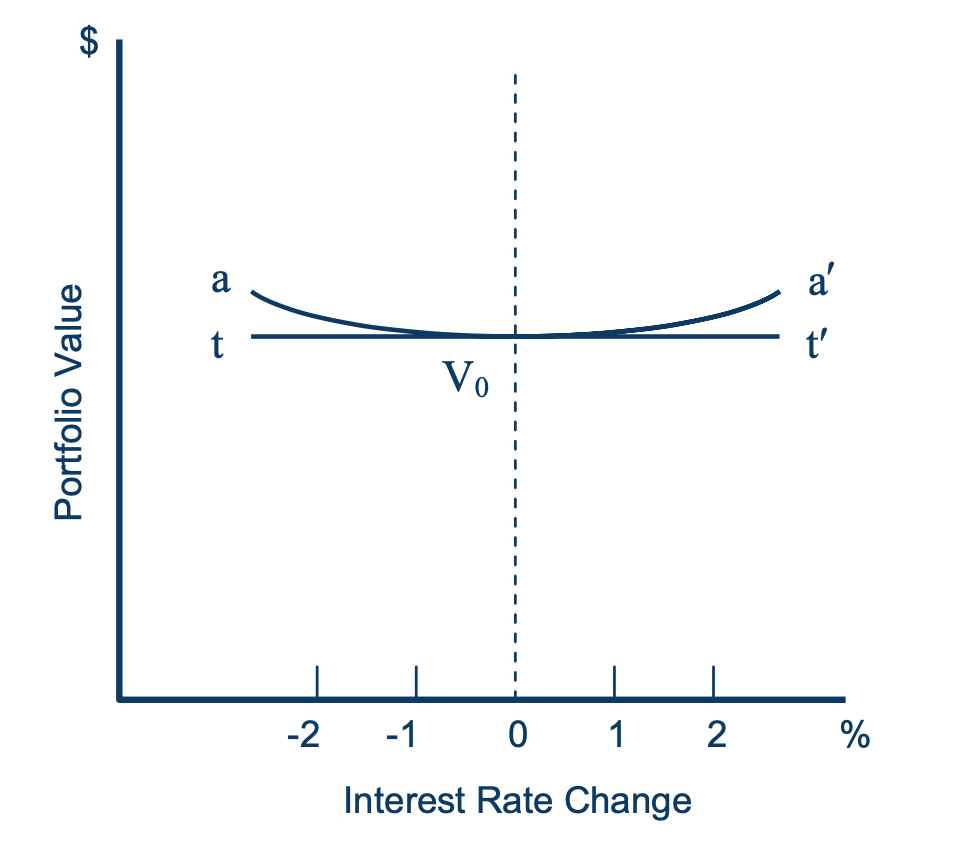
\includegraphics[width=12cm]{1}
\end{figure}

\begin{figure}[H]
\caption{Deux possibilités de changements de la valeur du portefeuille causés par des variations non parallèles des taux d'intérêt pour un portefeuille immunisé.}
\centering
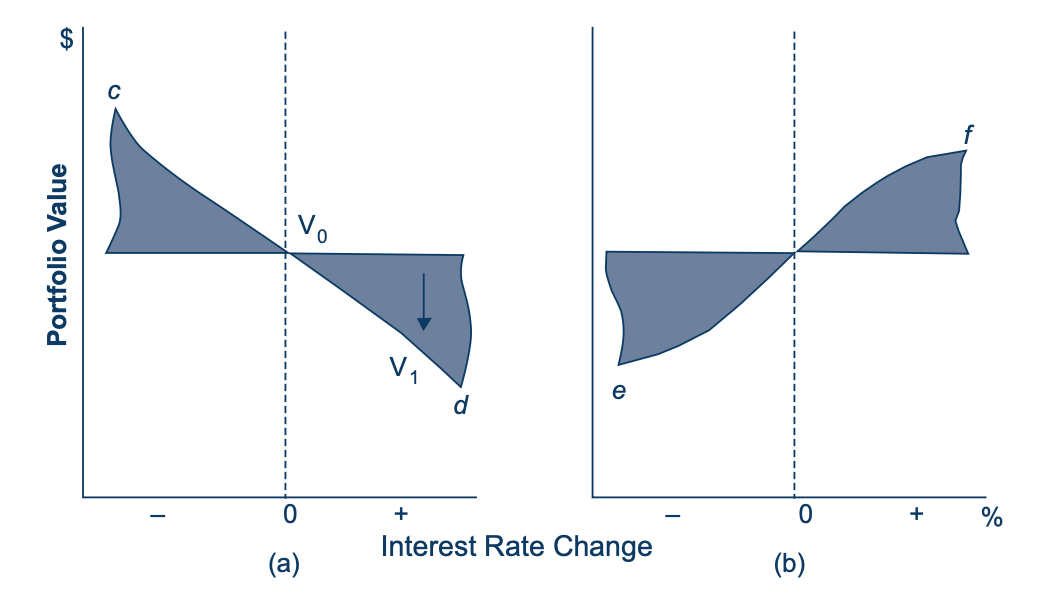
\includegraphics[width=14cm]{2}
\end{figure}

La figure 1 illustre la nature de la valeur du portefeuille, compte tenu d'un portefeuille immunisé et des variations parallèles des taux. La courbe $a-a^'$ représente le comportement de la valeur du portefeuille pour divers changements de taux, allant d'une baisse à une augmentation comme indiqué sur l'axe horizontal. Le point $V_0$ de la ligne $t-t^'$ est le niveau de la valeur du portefeuille en supposant l'absence de changement des taux.  Un portefeuille immunisé soumis à des déplacements parallèles de la courbe des taux fournira une valeur de portefeuille au moins aussi élevée à la date d'horizon que la valeur cible assurée, qui devient ainsi la valeur minimale. Par conséquent, si les hypothèses de la théorie classique sont valables, l'immunisation fournit une stratégie à risque minimum.

\vspace{0.5cm}


La figure 2 illustre la relation entre la valeur d'un portefeuille immunisé de façon classique et les variations des taux d'intérêt lorsque les taux d'intérêt ne changent pas de façon parallèle.  Selon la forme du décalage non parallèle, la relation indiquée en $a)$ ou celle illustrée en $b)$ se produira. Cette figure montre la possibilité (dans les cas $d$ et $e$) que la valeur d'un portefeuille immunisé de manière classique puisse être inférieure à la cible. Le point important est que le simple fait de faire correspondre la durée du portefeuille à l'horizon d'investissement comme condition d'immunisation ne peut pas empêcher des écarts importants par rapport à la valeur cible.

\vspace{0.5cm}

Une extension naturelle de la théorie classique de l'immunisation est d'étendre la théorie au cas de variations non parallèles des taux d'intérêt. Deux approches ont été adoptées.

\begin{enumerate}
\item La première approche a consisté à modifier la définition de la duration afin de permettre des changements non parallèles de la courbe des taux, tels que la duration multifonctionnelle (également appelée duration fonctionnelle ou duration des taux directeurs)
\item La deuxième approche est une stratégie qui peut gérer tout changement arbitraire de taux d'intérêt de sorte qu'il n'est pas nécessaire de spécifier une autre mesure de durée. Cette approche, développée par Fong et Vasicek (1984), établit une mesure du risque d'immunisation contre toute variation arbitraire des taux d'intérêt. La mesure du risque d'immunisation peut alors être minimisée sous réserve que la durée du portefeuille soit égale à l'horizon d'investissement, ce qui se traduit par un portefeuille avec une exposition minimale aux fluctuations des taux d'intérêt.
\end{enumerate}

\vspace{0.5cm}

Une deuxième extension de la théorie classique d'immunisation s'applique au dépassement des limites d'un horizon fixe (la deuxième hypothèse dont dépend l'immunisation). Marshall et Yawitz (1982) ont démontré que, dans l'hypothèse de variations parallèles des taux d'intérêt, une borne inférieure existe sur la valeur d'un portefeuille d'investissement à un moment donné, bien que cette borne inférieure puisse être inférieure à la valeur réalisée si les taux d'intérêt ne changent pas. Fong et Vasicek (1984) et Bierwag, Kaufman et Toevs (1979) ont étendu l'immunisation au cas des responsabilités multiples. L'immunisation à responsabilité multiple implique une stratégie d'investissement qui garantit le respect d'un calendrier spécifié de passifs futurs, quel que soit le type de changement dans les variations des taux d'intérêt. Fong et Vasicek (1984) ont fourni une généralisation de la mesure du risque d'immunisation pour le cas de responsabilité multiple.

\vspace{0.5cm}

La troisième extension de la théorie classique de l'immunisation consiste à analyser le compromis entre le risque et le rendement des portefeuilles immunisés. Fong et Vasicek (1983) ont montré comment ce compromis peut être analysé. Leur approche est appelée \textbf{maximisation du rendement}.

\vspace{0.5cm}

La quatrième extension de la théorie classique de l'immunisation consiste à intégrer des stratégies d'immunisation à des éléments de stratégies de gestion active de portefeuille obligataire. L'objectif traditionnel de l'immunisation a été la protection contre les risques, avec peu de considération pour les retours possibles. Leibowitz et Weinberger (1981) ont proposé une technique appelée immunisation contingente, qui offre une certaine souplesse dans la poursuite de stratégies actives tout en garantissant un certain rendement minimum dans le cas d'un changement de taux parallèle. Dans l'immunisation contingente, l'immunisation sert de stratégie de repli si le portefeuille géré activement ne croît pas à un certain rythme.

\section{Durée et convexité des actifs et des passifs}
Pour qu'un gestionnaire puisse avoir une image claire de l'excédent économique du portefeuille - défini comme la valeur marchande des actifs moins la valeur actuelle des passifs - la durée et la convexité des actifs et des passifs doivent être comprises. Se concentrer uniquement sur la durée des actifs d’une entreprise ne donnera pas une véritable indication du risque de taux d’intérêt total pour une entreprise.
\section{Types de risque}
À mesure que l'environnement de marché évolue, le gestionnaire de portefeuille court le risque de ne pas être en mesure de payer les dettes à leur échéance. Les trois sources de ce risque sont le risque de taux d'intérêt, le risque de réclamation conditionnelle et le risque de plafonnement.
\begin{enumerate}
\item \textbf{Risque de taux d'intérêt}: Étant donné que les prix de la plupart des titres à revenu fixe évoluent à l'opposé des taux d'intérêt, une hausse des taux d'intérêt aura une incidence défavorable sur la valeur d'un portefeuille. Si des actifs doivent être vendus pour assurer le service des passifs, le gestionnaire peut trouver un manque à gagner. Le risque de taux d'intérêt est le plus grand risque auquel un gestionnaire de portefeuille sera confronté.
\item \textbf{Risque de réclamations éventuelles}: Lorsqu'un titre comporte une disposition de réclamation conditionnelle, explicite ou implicite, il existe un risque associé. Dans un environnement de taux en baisse, le gestionnaire peut interrompre les paiements de coupons lucratifs et recevoir le principal (comme c'est le cas avec les titres adossés à des créances hypothécaires lorsque les prêts hypothécaires sous-jacents remboursent le principal).La perte des coupons est déjà assez grave, mais maintenant le principal doit être réinvesti à un taux inférieur. De plus, la valeur marchande d'un titre appelable se stabilisera au prix d'appel, plutôt que de continuer à augmenter comme le ferait un titre non remboursable.
\item \textbf{Risque de plafond}: Un actif qui effectue des paiements à taux variable aura généralement des plafonds associés au taux variable. Le gérant risque de voir le niveau des taux du marché augmenter alors que les rendements des actifs sont plafonnés. Cet événement peut affecter gravement la valeur des actifs.
\end{enumerate}

\section{Minimisation des risques pour les portefeuilles immunisés}
\begin{figure}[H]
\caption{Illustration de la mesure des risques liés à l'immunisation}
\centering
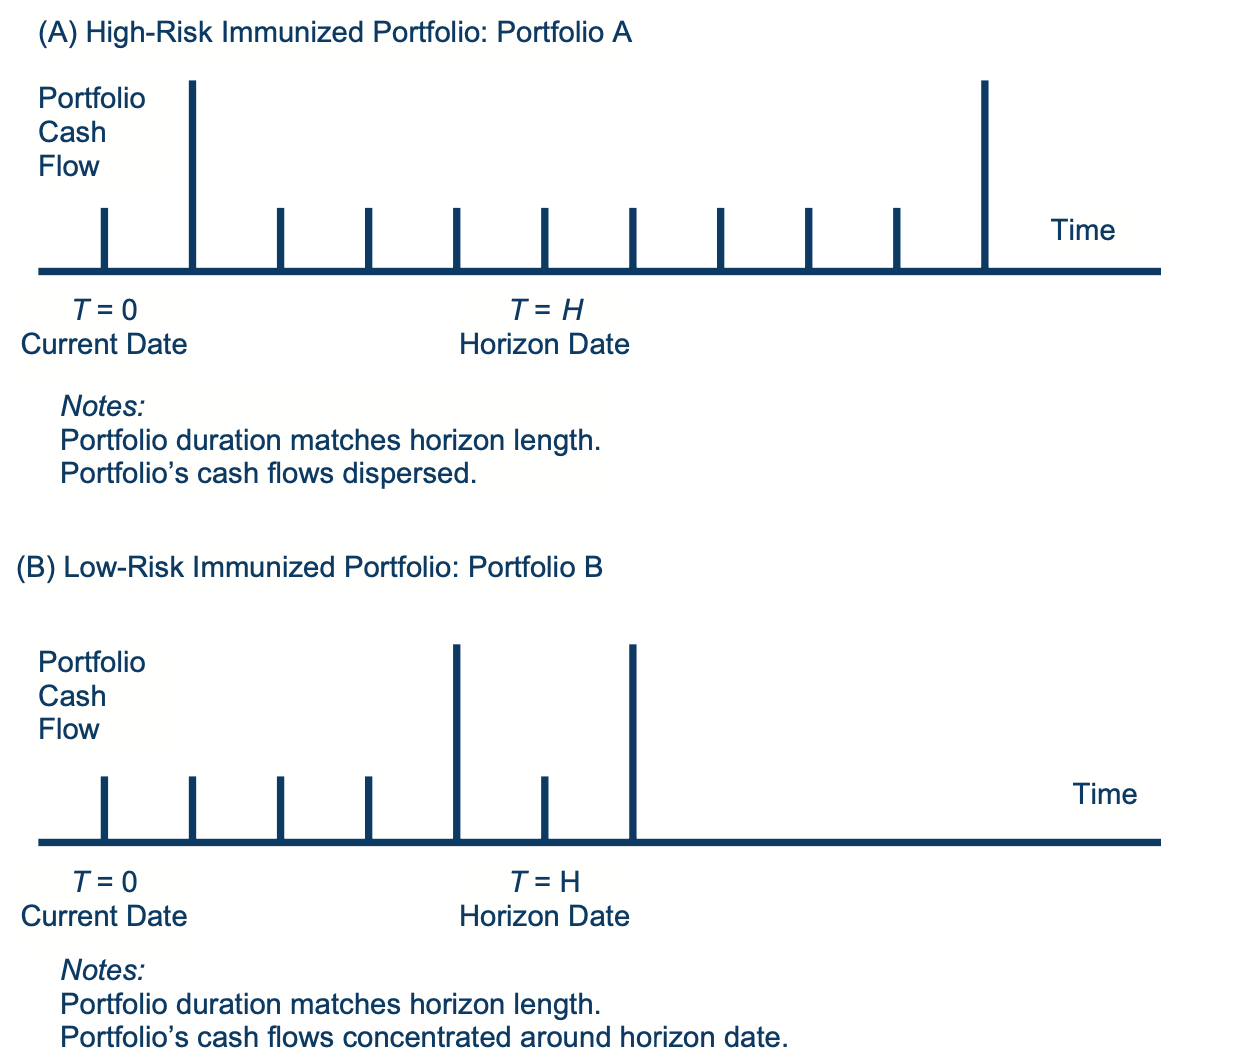
\includegraphics[width=14cm]{3}
\end{figure}

Dans la figure 3, les pics représentent les flux de trésorerie réels du portefeuille. Les pics les plus élevés représentent les flux de trésorerie réels générés par les titres à l'échéance, tandis que les pics plus petits représentent les paiements de coupons. Le portefeuille A et le portefeuille B sont tous deux composés de deux obligations dont la durée est égale à l'horizon d'investissement. Le portefeuille A est, en fait, un portefeuille haltère (un portefeuille composé d'échéances courtes et longues par rapport à la date d'horizon et des paiements de coupons intermédiaires). Le portefeuille B, cependant, est un portefeuille de bullet (les échéances des obligations sont très proches de l'horizon d'investissement). Si les deux portefeuilles ont des durées égales à la longueur de l'horizon, les deux portefeuilles sont immunisés contre des variations de taux parallèles. Cependant, lorsque les taux d'intérêt changent de manière arbitraire et non parallèle, l'effet sur la valeur des deux portefeuilles diffère )(le portefeuille haltères est plus risqué que le portefeuille bullet).

\vspace{0.5cm}

Si les taux courts terme baissent tandis que les taux longs terme augmentent :
\begin{itemize}
\item Les portefeuilles haltères et bullet réaliseraient une baisse de la valeur du portefeuille à la fin de l'horizon de placement sous la valeur de placement cible, car ils subiraient une perte en capital en plus de taux de réinvestissement plus faibles.
\item La baisse serait toutefois nettement plus élevée pour le portefeuille d'haltères
\begin{itemize}
\item Le portefeuille d'haltères connaît des taux de réinvestissement plus bas plus longtemps que le portefeuille de bullet
\item Une plus grande partie du portefeuille haltères est toujours en souffrance à la fin de l'horizon de placement, ce qui signifie que la même augmentation de taux entraîne beaucoup plus de perte en capital.
\end{itemize}
En bref, le portefeuille bullet est moins exposé aux variations de la structure des taux d'intérêt que le portefeuille haltères.

\section{Stratégies d'appariement des flux de trésorerie}
L'appariement des flux de trésorerie est une alternative à l'immunisation de responsabilité multiple dans la gestion actif / passif. L'appariement des flux de trésorerie est une stratégie attrayante car le gestionnaire de portefeuille n'a besoin que de sélectionner des titres qui correspondent au moment et au montant des passifs. Conceptuellement, une obligation est sélectionnée avec une échéance qui correspond au dernier passif, et un montant de principal égal au montant du dernier passif moins le paiement final du coupon est investi dans cette obligation. Les éléments restants du flux de passif sont ensuite réduits des paiements de coupon sur cette obligation, et une autre obligation est choisie pour l'avant-dernier passif, ajustée pour tout paiement de coupon reçu sur la première obligation sélectionnée. En remontant dans le temps, cette séquence se poursuit jusqu'à ce que tous les passifs aient été compensés par des paiements sur les titres sélectionnés pour le portefeuille. Des techniques de programmation linéaire peuvent être utilisées pour construire un portefeuille d'appariement de flux de trésorerie au moindre coût à partir d'un univers d'obligations acceptable. La figure 4 fournit une illustration simple de ce processus pour un volet de responsabilité de cinq ans.


\begin{figure}[H]
\caption{Illustration du processus d'appariement des flux de trésorerie}
\centering
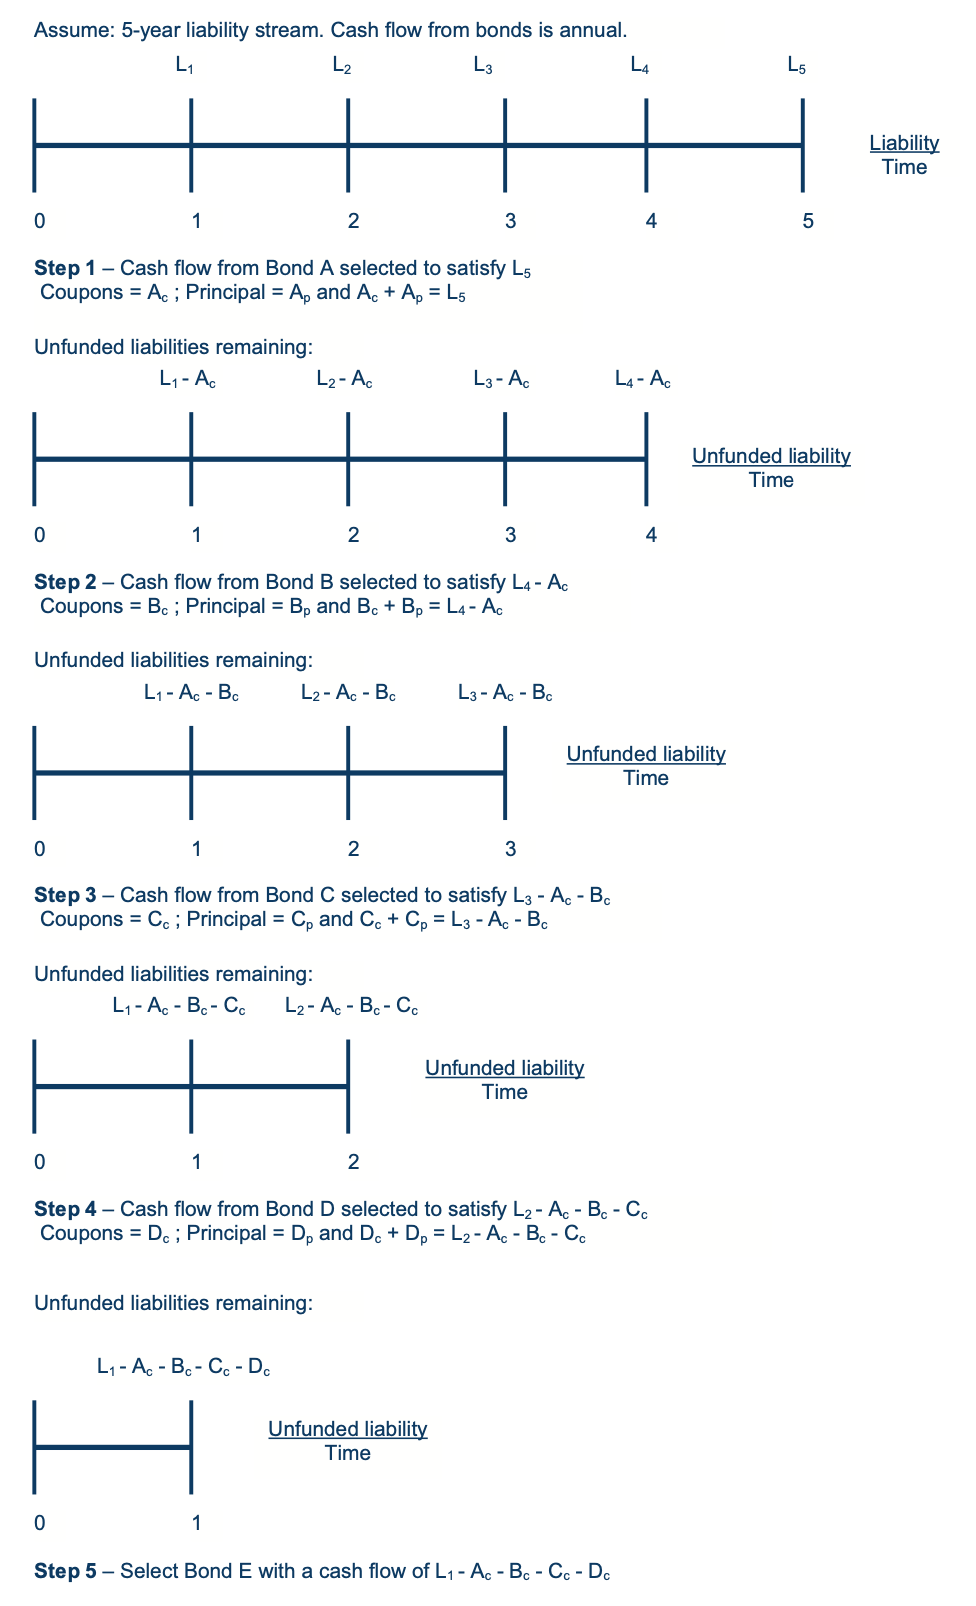
\includegraphics[width=14cm]{4}
\end{figure}

\section{Exemples}
\subsection{Question 1}
Le tableau ci-dessous présente le rendement actif sur six périodes d'un portefeuille obligataire. Calculez le portfolio’s tracking risk pour la période de six périodes.

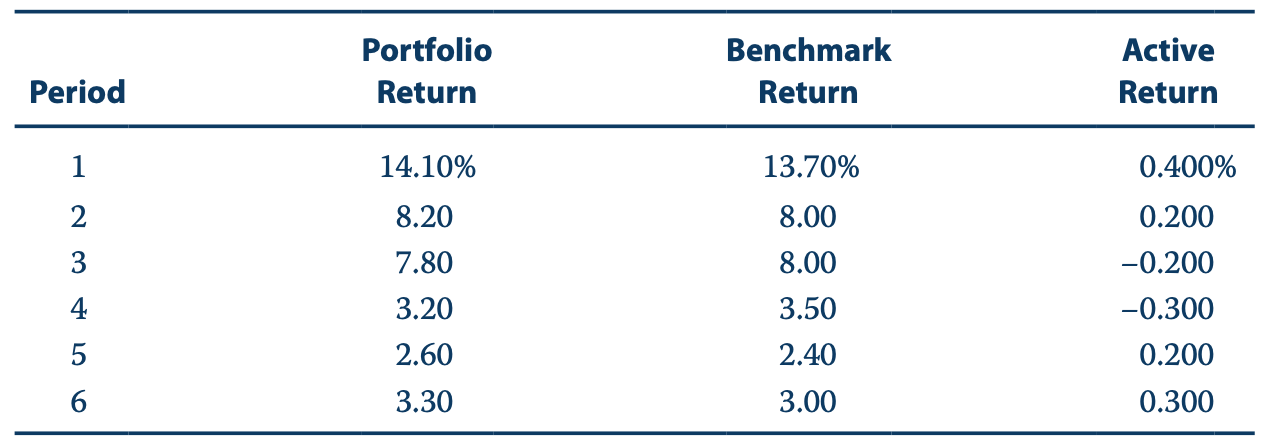
\includegraphics[width=14cm]{5}

\textbf{Le tracking risk est l'écart type des rendements actifs. Pour les données présentées dans le problème, le tracking risk  est de 28,284 point de base.}

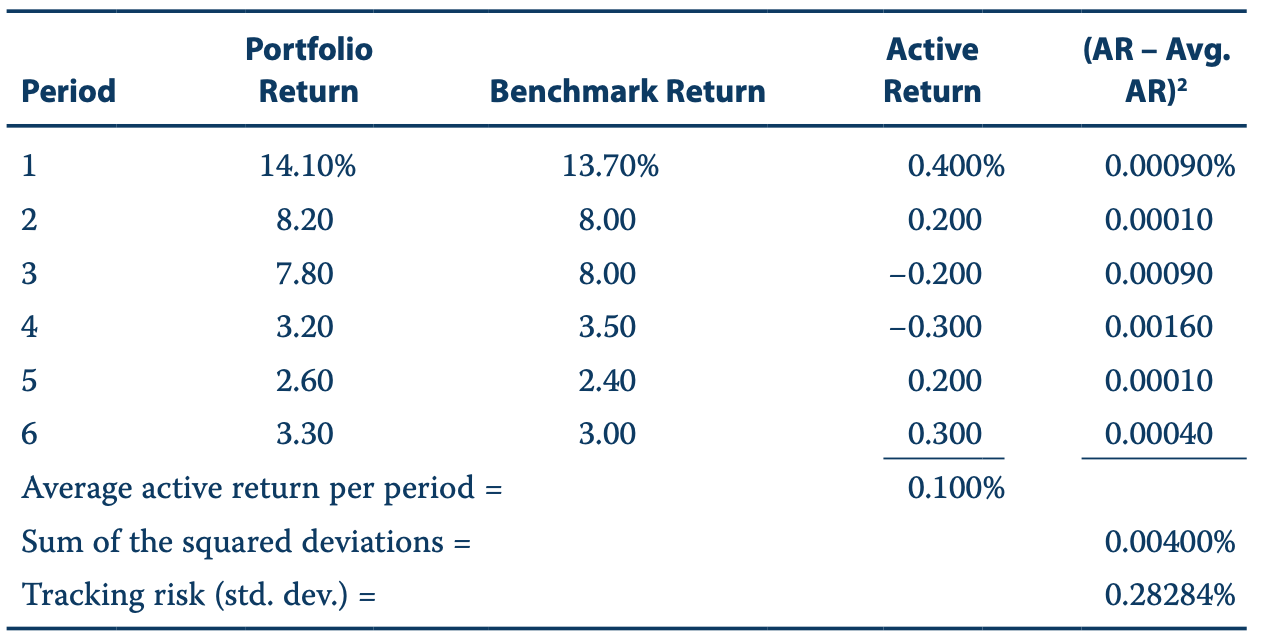
\includegraphics[width=14cm]{6}

\newpage

\subsection{Question 2}
Le tableau ci-dessous présente la duration du spread pour un portefeuille de 70 obligations et un indice de référence basé sur les secteurs. Déterminez si le portefeuille ou l'indice de référence est plus sensible aux variations du spread sectoriel en déterminant la duration du spread pour chacun. Compte tenu de votre réponse, quel est l’effet sur le portfolio’s tracking risk?

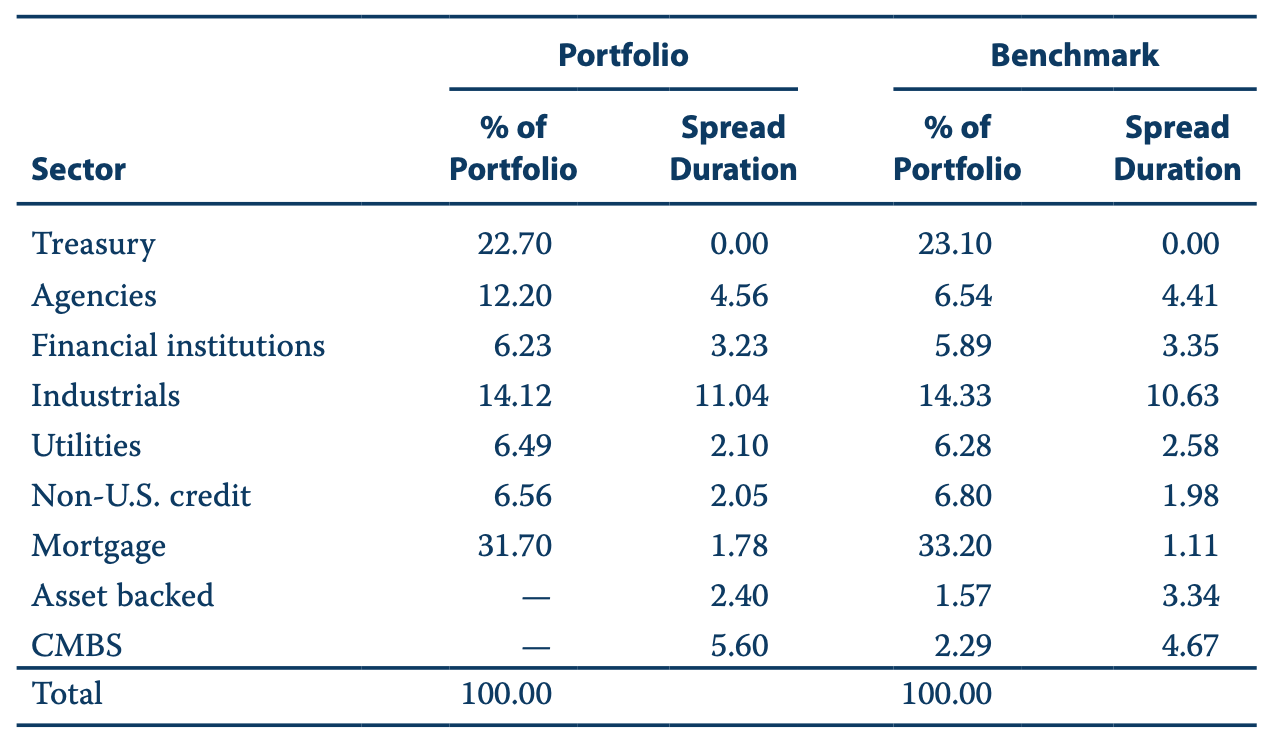
\includegraphics[width=14cm]{7}

\textbf{Le portefeuille est plus sensible aux variations du spread car sa duration du spread est de 3,151 par rapport à 2,834 de l’indice de référence. La durée plus élevée du spread du portefeuille est principalement attribuable au poids plus important du portefeuille sur les titres d’agence. La durée du spread pour chacun peut être calculée en prenant une moyenne pondérée des durées des différents secteurs. Puisqu'il existe une différence entre la duration du spread du portefeuille et celle de l'indice de référence,  le tracking risk sera plus élevé que si les deux étaient plus étroitement appariés.}

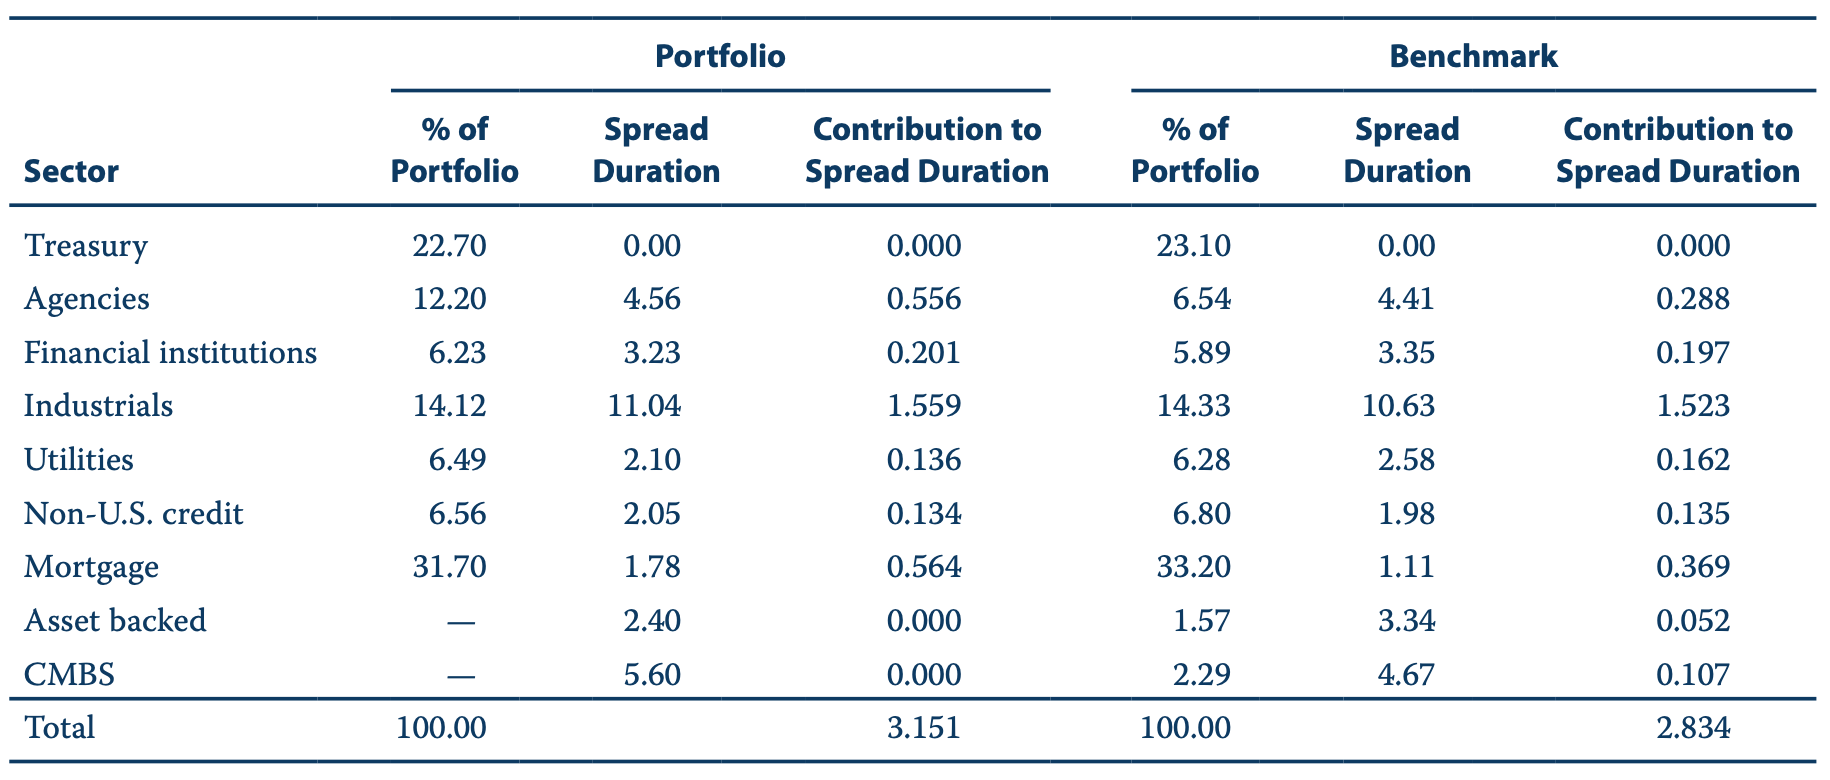
\includegraphics[width=16cm]{8}

\newpage

\subsection{Question 3}
Vous êtes le gestionnaire d'un portefeuille composé de trois obligations d'un montant nominal égal de 1 000 000 \$ chacune. Le premier tableau ci-dessous montre la valeur de marché des obligations et leurs durées. (Le prix comprend les intérêts courus.) Le deuxième tableau contient la valeur marchande des obligations et leur durée un an plus tard.

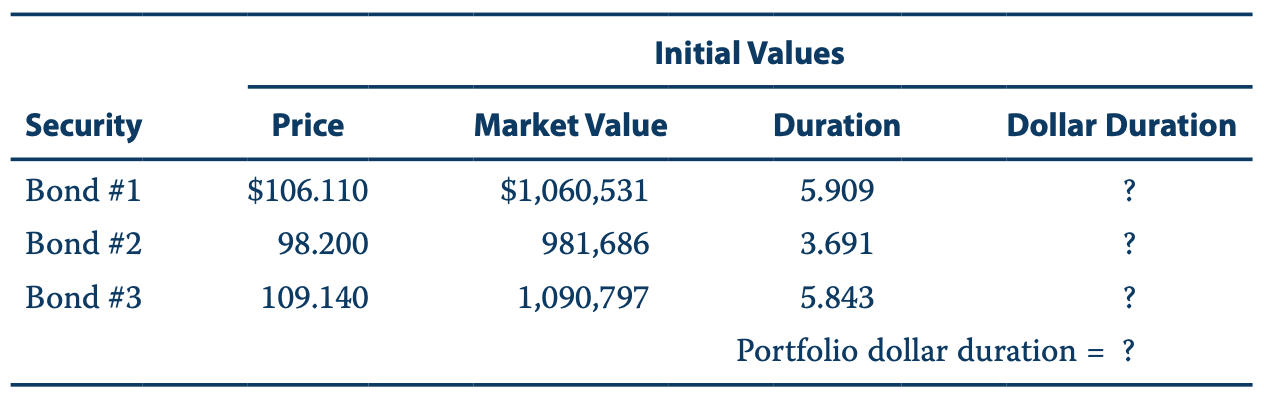
\includegraphics[width=14cm]{9}

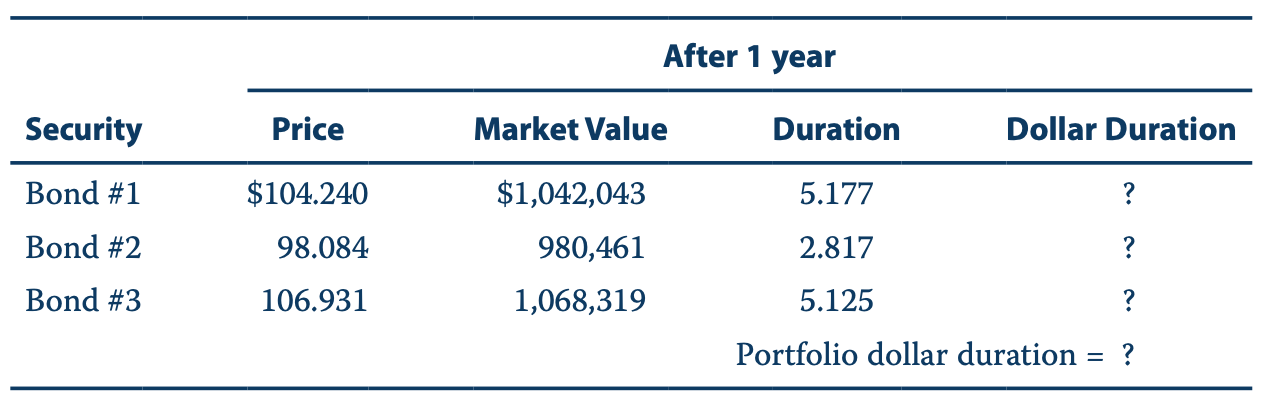
\includegraphics[width=14cm]{10}

En tant que gestionnaire, vous souhaitez maintenir la duration en dollars du portefeuille au niveau initial en rééquilibrant le portefeuille. Vous choisissez de rééquilibrer en utilisant les proportions de sécurité existantes d'un tiers chacune.  Calculer:
\begin{enumerate}
\item les durées en dollars de chacune des obligations.
\item le taux de rééquilibrage nécessaire au rééquilibrage.
\item les liquidités nécessaires au rééquilibrage.
\end{enumerate}

La duration en dollars est une mesure de la variation de la valeur du portefeuille pour une variation de 100 point de base des rendements du marché.  La duration en dollars d’un portefeuille est la somme des durées en dollars des titres qui le composent. La duration en dollars de ce portefeuille au début de la période est de 162636 \$.

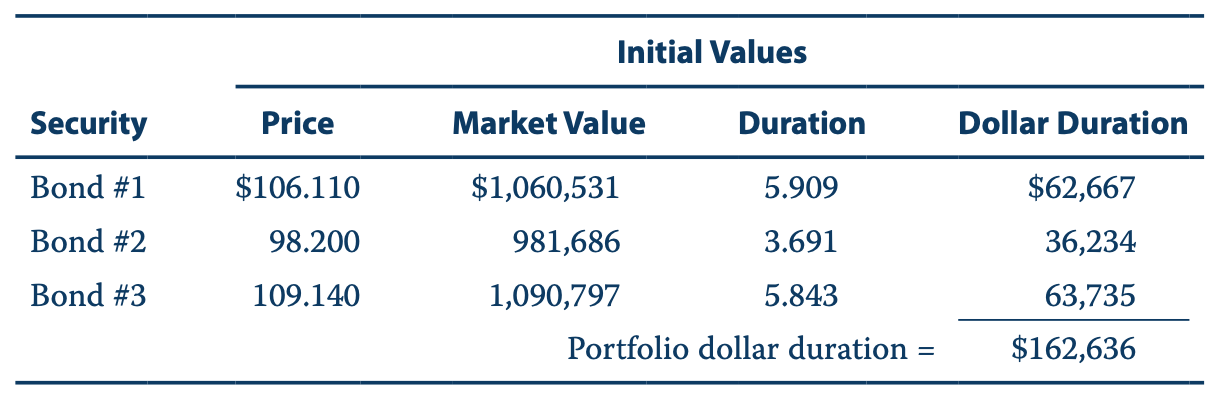
\includegraphics[width=14cm]{11}


À la fin d’un an, la duration en dollars du portefeuille est passée à 136 318 \$

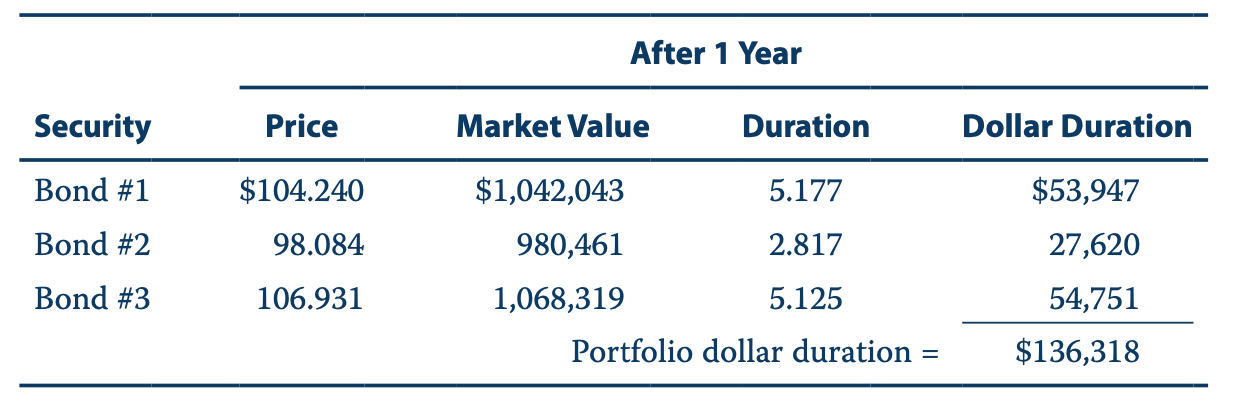
\includegraphics[width=14cm]{12}

Le ratio de rééquilibrage est un ratio de la durée d'origine en dollars sur la nouvelle durée en dollars:
\begin{align*}
\textbf{Rebalancing ratio} =\frac{162636}{136318} = 1.193
\end{align*}

Le portefeuille exige que chaque position soit augmentée de 19,3\%. La trésorerie nécessaire à ce rééquilibrage est calculée comme suit:

\begin{align*}
\textbf{Cash required} = 0.193 × (1042043 + 980461 + 1068319)=596529
\end{align*}

\newpage

\subsection{Question 4}
Le comité d'investissement de l'Université de Rojas est mécontent de la performance récente de la partie à revenu fixe de sa dotation et a licencié l'actuel gestionnaire de titres à revenu fixe. Le portefeuille actuel, comparé à l'indice Lehman Brothers U.S. Aggregate, est présenté dans le tableau suivant. Le comité d’investissement engage Alfredo Alonso, un consultant de MHC Consulting, pour évaluer les risques du portefeuille, soumettre des idées au comité et gérer le portefeuille de manière intérimaire.

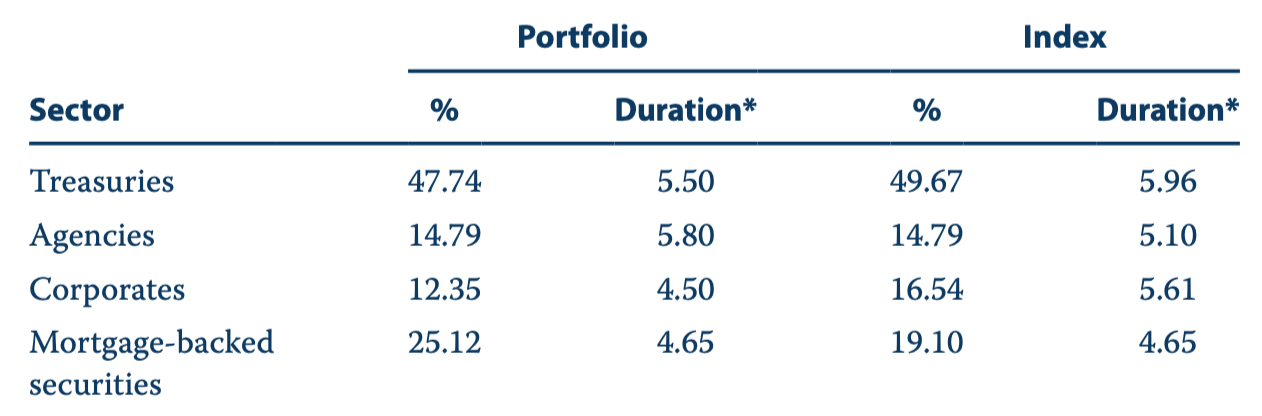
\includegraphics[width=14cm]{13}

Alonso remarque que le portefeuille du gestionnaire licencié ne détenait pas de titres en dehors de l’univers de l’indice. Le comité demande à Alonso d'envisager une stratégie d'indexation, y compris les avantages connexes et les problèmes logistiques. Alonso identifie trois facteurs qui limitent la capacité d'un gestionnaire à répliquer un indice obligataire:
\begin{enumerate}
\item Un manque de disponibilité de certaines émissions obligataires
\item Un manque de données indicielles disponibles pour positionner le portefeuille
\item Différences entre les prix des obligations utilisés par le gestionnaire et le fournisseur de l'indice
\end{enumerate}
Alonso a effectué une analyse plus approfondie de la portion actuelle du Trésor américain du portefeuille et a découvert une surpondération importante dans un bon du Trésor à 5 ans (valeur nominale de 10 millions de dollars). Il s'attend à ce que la courbe des taux s'aplatisse et prévoit un prix à l'horizon de six mois du bon du Trésor à 5 ans à 99,50 \$. Par conséquent, la stratégie d’Alonso consistera à vendre tous les bons du Trésor à 5 ans et à investir le produit dans des bons du Trésor à 10 ans et des liquidités tout en maintenant la duration en dollars du portefeuille. Les informations sur les obligations du Trésor américain sont présentées dans le tableau suivant:

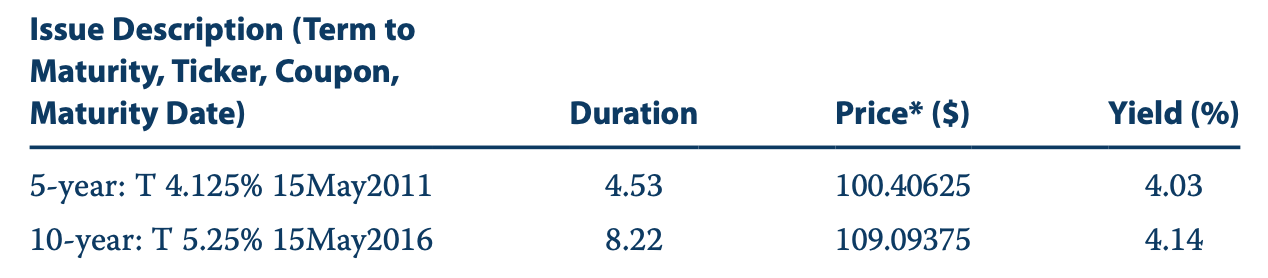
\includegraphics[width=14cm]{14}

\vspace{0.5cm}

\subsubsection*{Quelle est la durée du portefeuille de titres à revenu fixe de l'Université Rojas ?}
La durée du portefeuille est une moyenne pondérée des durées des obligations individuelles.
\begin{align*}
(0.4774 \times 5.50) + (0.1479 \times 5.80) + (0.1235 \times 4.50)+ (0.2512 \times 4.65) = 5.20735
\end{align*}

La durée du portefeuille est de 5.20735

\subsubsection*{Quelle est la stratégie de portefeuille obligataire utilisée par le gestionnaire licencié ?}
\begin{itemize}
\item Les pondérations du portefeuille diffèrent considérablement pour certains secteurs de celles de l'indice
\item Les durées des composantes du portefeuille diffèrent de leurs durées respectives dans l'indice.
\item Le gestionnaire utilise une gestion active car il permet un décalages de la durée et du secteur.
\end{itemize}

\subsubsection*{En ce qui concerne les trois facteurs identifiés par Alonso, quel est le facteur le moins susceptible de limiter la capacité d’un gestionnaire à répliquer un indice obligataire ?}
 Les données d'index sont facilement disponibles. Alonso a tort d'identifier cela comme un facteur limitant. Les informations (données) pour les deux autres facteurs peuvent être difficiles, voire impossibles à acquérir.
\subsubsection{Quelle est la valeur nominale des obligations à 10 ans à acheter pour exécuter la stratégie d’Alonso ?}
Alonso ne va pas simplement réinvestir l'intégralité du produit de la vente dans des bons du Trésor à 10 ans, car son désir déclaré est de maintenir la duration en dollars du portefeuille. Le prix de vente de 10 millions de dollars de la valeur nominale de l'obligation de 5 ans est obtenu en multipliant $10000000 \times 1.0040625 = 10040625$ . La durée en dollars de la période de 5 ans est de $4,53 \times 10040625 \times 0.01 = 454840.31$ . Divisez maintenant 454 840.31  par le produit de la durée du 10 ans et de son prix coté et 0.01 pour obtenir la valeur nominale du 10 ans. Le résultat est $454840.31  / (8,22 \times 1,0909375 \times 0.01) = 5072094$.
\end{document}